\documentclass{article}
\usepackage[left=4cm, right=3cm, top=3cm, bottom=3cm]{geometry}
\usepackage{amsmath}
\usepackage[hidelinks]{hyperref}
\DeclareMathOperator*{\argmax}{\arg\!\max}
\usepackage{amssymb}
\usepackage[utf8]{inputenc}
\usepackage{graphicx}
\graphicspath{{../images/}}
\usepackage{csquotes}
\usepackage[font={small, it}]{caption}

\title{Notes \\ Reinforcement Learning: An Introduction (2\textsuperscript{nd} Edition)}
\author{Scott Jeen}
\date{\today}

\begin{document}
	
\maketitle
\tableofcontents
\section{Introduction }	
\subsection{Overview}
\begin{itemize}
	\item Supervised learning = learning with labels defined by human; Unsupervised learning = finding patterns in data. Reinforcement learning is a 3rd machine learning paradigm, in which the agent tries to maximise its reward signal.
	\item Exploration versus exploitation problem - agent wants to do what it has already done to maximise reward by exploitation, but there may be a bigger reward available if it were to explore.
	\item RL is based on the model of human learning, similar to that of the brain's reward system.
\end{itemize}

\subsection{Elements of Reinforcement Learning}
\begin{description}
	\item[Policy] Defines the agent's way of behaving at any given time. It is a mapping from the perceived states of the environment to actions to be taken when in those states.
	\item[Reward Signal] The reward defines the goal of the reinforcement learning problem. At each time step, the environment sends the RL agent a single number, a \textit{reward}. It is the agent's sole objective to maximise this reward. In a biological system, we might think of rewards as analogous to pain and pleasure. The reward sent at any time depends on the agent's current action and the agent's current state. If my state is hungry and I choose the action of eating, I receive positive reward.
	\item[Value function] Reward functions indicate what is good immediately, but value functions specify what is good in the long run. The value function is the total expected reward an agent is likely to accumulate in the future, starting from a given state. E.g. a state might always yield a low immediate reward, but is normally followed by a string of states that yield high reward. Or the reverse. Rewards are, in a sense, primary, whereas values, as predictions of rewards, are secondary. Without rewards there could be no value. Nevertheless, it is values with which we are most concerned when evaluating decisions. We seek actions that bring the highest value, not the highest reward, because they obtain the greatest amount of reward over the long run. Estimating values is not trivial, and efficiently and accurately estimating them is the core of RL.
	\item[Model of environment (optionally)] Something that mimics the behaviour of the true environment, to allow inferences to be made about how the environment will behave. Given a state and action, the model might predict the resultant next state and next reward. They are used for \textit{planning}, that is, deciding on a course of action by considering possible future situations before they are actually experienced. 
\end{description}

	
	
	
	

\section{Multi-arm Bandits}

RL evaluates the actions taken rather than instructs correct actions like other forms of learning.

\subsection{An n-Armed Bandit Problem}
\textbf{The problem}
\begin{itemize}
\item You are faced repeatedly with a choice of \textit{n} actions.
\item After each choice, you receive a reward from a stationary probability distribution.
\item Objective is to maximise total reward over some time period, say 100 time steps.
\item Named after of slot machine (one-armed bandit problem), but \textit{n} levers instead of 1.
\item Each action has an expected or mean reward based on its probability distribution. We shall call thjs the \textit{value} of the action. We do not know these values with certainty.
\item Because of this uncertainty, there is always an exploration vs exploitation problem. We always have one action that we deem to be most valuable at any instant, but it is highly likely, at least initially, that there are actions we are yet to explore that are more valuable.
\end{itemize}

\subsection{Action-Value Methods}
The estimated action value is
\begin{equation} \label{eq: estimated value}
	Q_t(a) = \frac{R_1+R_2+\cdots+R_{N_t(a)}}{N_t(a)}
\end{equation}

The true value (mean reward) of an action is \(q\), but the estimated value at the \textit{t}th time-step is Q(a), given by Equation \ref{eq: estimated value} (our estimate after \textit{N} selections of an action yielding \textit{N} rewards).\\

The greedy action selection method is
\begin{equation} \label{eq: argmax}
A_t =\argmax_a Q_t(a)
\end{equation}

\begin{itemize}
	\item Simplest action selection rule is to select the action with the highest estimated value.
	\item $\argmax_a$ means the value of \(a\) for which \(Q_t\) is maximised.
	\item \(\epsilon\)-greedy methods are where the agent selects the greedy option most of the time, and selects a random action with probability \(\epsilon\).
	\item Three algorithms are tried: one with \(e\)=0 (pure greedy), one with \(e\)=0.01 and another with \(e\)=0.1
	\item Greedy method gets stuck performing sub-optimal actions.
	\item \(e\)=0.1 explores more and usually finds the optimal action earlier, but never selects it more that 91\% of the time.
	\item \(e\)=0.01 method improves more slowly, but eventually performs better than the e=0.1 method on both performance measures.
	\item It is possible to reduce \(e\) over time to try to get the best of both high and low values.
\end{itemize}
\begin{figure}
	\centering
	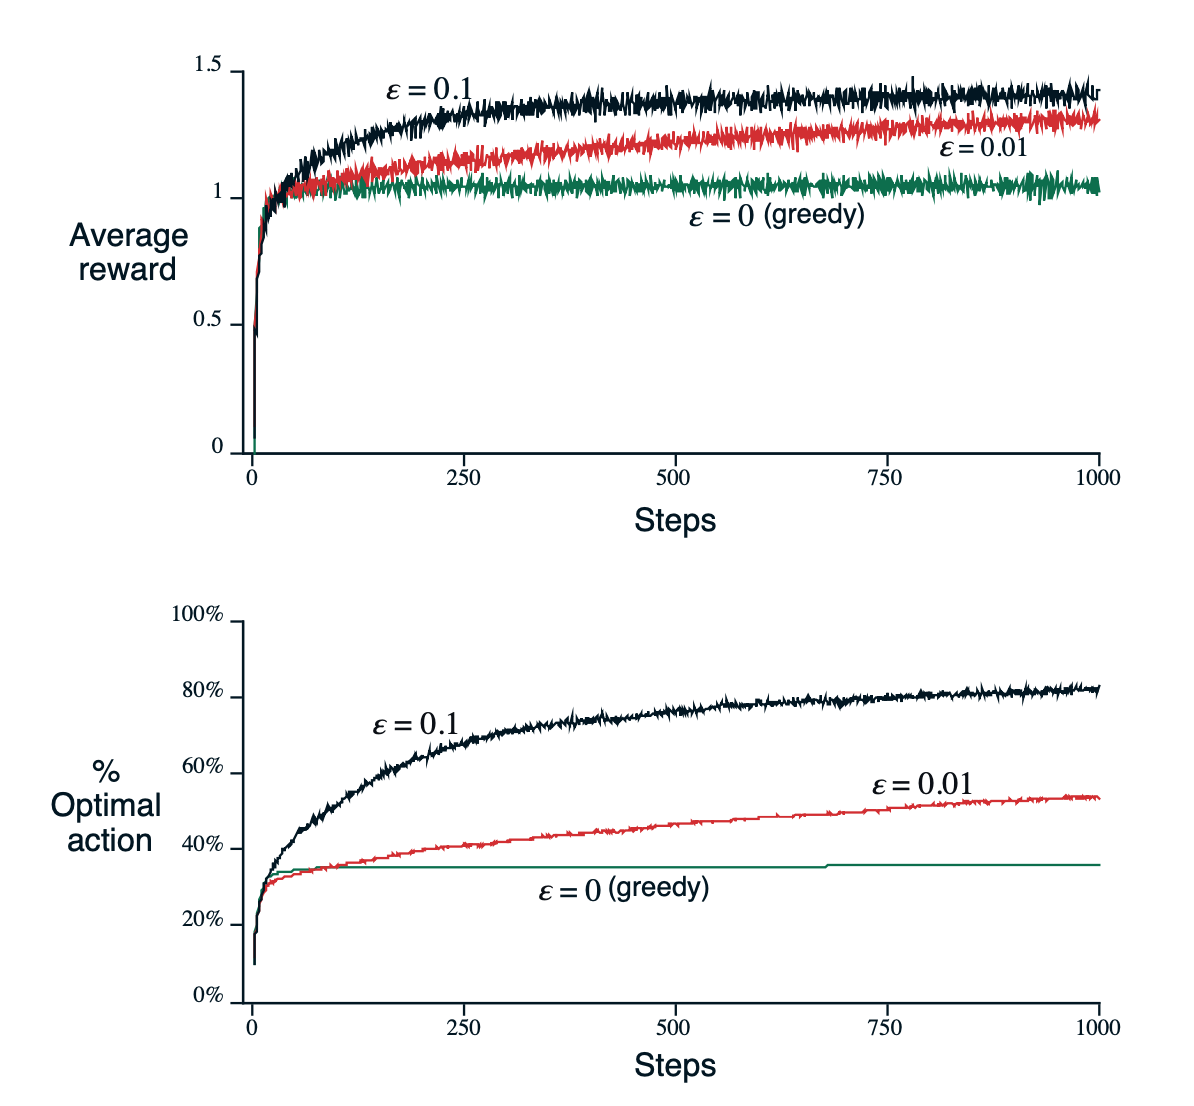
\includegraphics[width=0.8\textwidth]{/chapter2_1}
	\caption{Average performance of $\epsilon$-greedy action-value methods on the 10-armed testbed. These data are averages over 2000 runs with different bandit problems. All methods used sample averages as their action-value estimates.}
	\label{fig:chapter2_1}
\end{figure}

\subsection{Incremental Implementation}
The sample-average technique used to estimate action-values above has a problem: memory and computation requirements grow over time. This isn't necessary, we can devise an incremental solution instead:

\begin{align}
	Q_{k+1} &= \frac{1}{k}\sum_{i}^{k}R_i \nonumber \\
	&= \frac{1}{k} \left( R_k + \sum_{i=1}^{k-1} R_i \right) \nonumber \\
	&= \vdots \\
	&= Q_k + \frac{1}{k} \left[R_k - Q_k\right] \\
\end{align}

We are updating our estimate of \(Q_{k+1}\) by adding the discounted error between the reward just received and our estimate for that reward \(Q_k\).

\begin{equation}
NewEstimate \leftarrow OldEstimate + StepSize \left[Target - OldEstimate \right]
\end{equation}

\(\alpha\) is used to denote the stepsize (\(\frac{1}{k}\)) in the rest of this book.

\subsection{Tracking a Nonstationary Problem}
The averaging methods discussed above do not work if the bandit is changing over time. In such cases it makes sense to weight recent rewards higher than long-past ones. The popular way of doing this is by using a constant step-size parameter.

\begin{equation}
	Q_{k+1} = Q_k +\alpha \left[R_k - Q_k\right]
\end{equation}

where the step-size parameter \(\alpha \in (0,1]\) is constant. This results in \(Q_{k+1}\) being a weighted average of the past rewards and the initial estimate \(Q_1\):

\begin{align}
Q_{k+1} &= Q_k +\alpha \left[R_k - Q_k\right] \nonumber \\
&= \alpha R_k + (1 - \alpha)Q_k \nonumber \\
&= \alpha R_k + (1 - \alpha)[\alpha R_{k-1} + (1 - \alpha)Q_{k-1}] \nonumber \\
&= \alpha R_k + (1 - \alpha)\alpha R_{k-1} + (1 - \alpha)^2 Q_{k-1}  \nonumber \\
&= \vdots \nonumber \\
&= (1-\alpha)^k Q_1 + \sum_{i}^{k} \alpha (1 - \alpha)^{k-i} R_i \\
\end{align}

\begin{itemize}
\item Because the weight given to each reward depends on how many rewards ago it was observed, we can see that more recent rewards are given more weight. Note the weights \(\alpha\) sum to 1 here, ensuring it is indeed a weighted average where more weight is allocated to recent rewards.
\item In fact, the weight given to each reward decays exponentially into the past. This sometimes called an \textit{exponential} or \textit{recency-weighted} average.
\end{itemize}

\subsection{Optimistic Initial Values}
\begin{itemize}
\item The methods discussed so far are dependent to some extent on the initial action-value estimate i.e. they are biased by their initial estimates.
\item For methods with constant \(\alpha\) this bias is permanent.
\item In effect, the initial estimates become a set of parameters for the model that must be picked by the user.
\item In the above problem, by setting initial values to +5 rather than 0 we encourage exploration, even in the greedy case. The agent will almost always be disappointed with it's samples because they are less than the initial estimate and so will explore elsewhere until the values converge.
\item The above method of exploration is called \textit{Optimistic Initial Values}.
\end{itemize}

\subsection{Upper-confidence-bound Action Selection}
\(\epsilon\)-greedy action selection forces the agent to explore new actions, but it does so indiscriminately. It would be better to select among non-greedy actions according to their potential for actually being optimal, taking into account both how close their estimates are to being maximal and the uncertainty in those estimates. One way to do this is to select actions as:

\begin{equation}
	A_t = \argmax_a \left[Q_t(a) + c\sqrt{\frac{\ln t}{N_t(a)}}\right]
\end{equation}

where c \(>\) 0 controls the degree of exploration.

\begin{itemize}
	\item The square root term is a measure of the uncertainity in our estimate. It is proportional to \(t\) i.e. how many timesteps have passed and inversely proportional to \(N_t(a)\) i.e. how many times that action has been visited. The more time has passed, and the less we have sampled an action, the higher our upper-confidence-bound.
	\item As the timesteps increases, the denominator dominates the numerator as the ln term flattens.
	\item Each time we select an action our uncertainty decreases because N is the denominator of this equation.
	\item UCB will often perform better than e-greedy methods
\end{itemize}

\begin{figure}
	\centering
	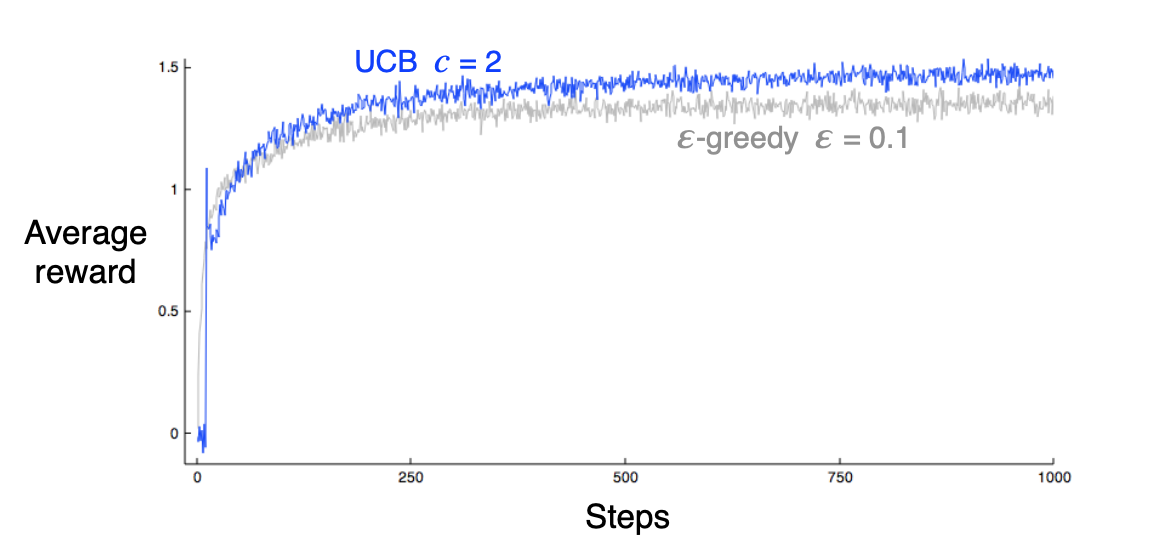
\includegraphics[width=0.8\textwidth]{/chapter2_2}
	\caption{UCB performs better than \(e\)-greedy in the n-armed bandit problem}
	\label{fig:chapter2_2}
\end{figure}

\subsection{Associative Search (Contextual Bandits)}
Thus far we have been discussing the stationary $k$-armed bandit problem, where the value of each arm is unknown but nonetheless remains stationary. Now, we consider a problem where the task could change from step to step, but the value distributions of the arms in each task remain the same. This is called contextual bandits, and in the toy example we are usually given a hint that the task has changed e.g. the slot machine changes colour for each task. Now we want to learn the correct action to take in a particular setting, given the task colour observed. This is an intermediary between the stationary problem and the full reinforcement learning problem. See exercise 2.10 below.

\subsection{Key Takeaways}
\begin{itemize}
\item The value of an action can be summarised by \(Q_t(a)\), the sample average return from an action
\item When selecting an action, it is preferable to maintain exploration, rather than only selecting the action we believe to be most valuable at any given timestep, to ensure we continue to improve our best estimate of the optimal action. We do so using \(\epsilon\))-greedy policies.
\item If our problem is non-stationary, rather than taking a standard average of every return received after an action, we can take a weighted average that gives higher value to more recently acquired rewards. We call this an \textit{exponential} or \textit{recency-weighted} average.
\item Optimistic initial values encourage lots of early exploration as our returns always decrease our estimate of \(Q_t\) meaning the greedy actions remain exploratory. Only useful for stationary problems.
\item \(\epsilon\)-greedy policies can be adapted to give more value to actions that have been selected less-often, i.e. actions where we have higher uncertainty in their value, using \textit{upper-confidence-bound} action selection.
\item Lastly, each of these techniques have varied performance on the n-armed bandit test dependent on their parametrisation. Their performance is plotted in Figure \ref{fig:chapter2_4}.
\end{itemize}

\begin{figure}
	\centering
	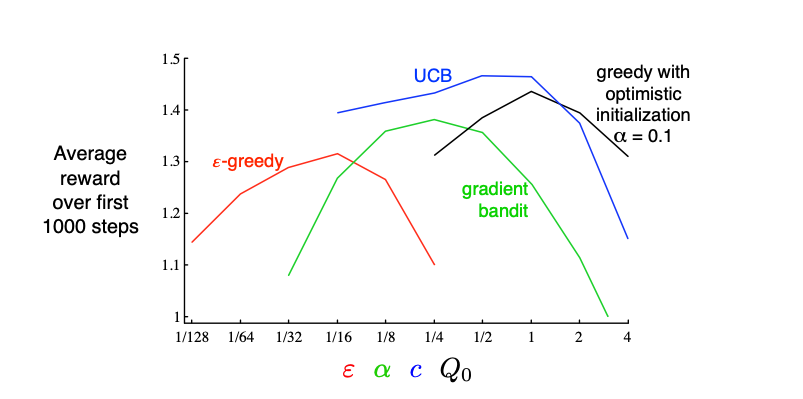
\includegraphics[width=0.8\textwidth]{/chapter2_4}
	\caption{Performance of each of the bandit algorithms explored in this chapter}
	\label{fig:chapter2_4}
\end{figure}


\section{Finite Markov Decision Processes}

\subsection{The Agent-Environment Interface}
\begin{figure}[h!]
	\centering
	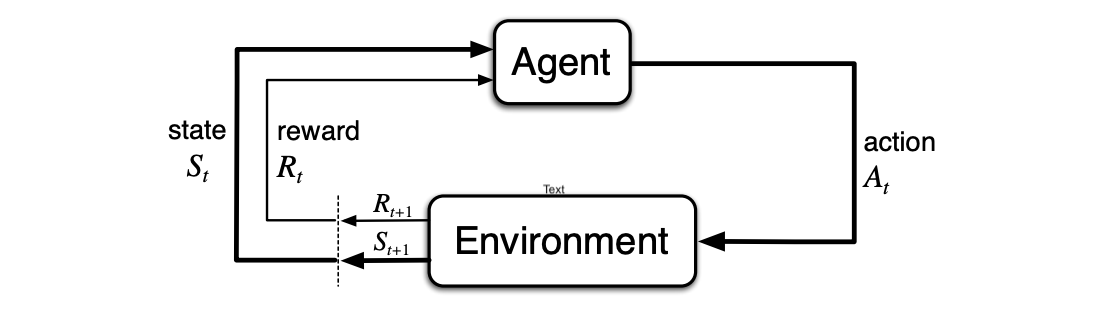
\includegraphics[width=\textwidth]{/chapter3_1}
	\caption{The agent-environment interface in reinforcement learning}
	\label{fig:agent-environment}
\end{figure}

\begin{itemize}
	\item At each timestep the agent implements a mapping from states to probabilities of selecting a possible action. The mapping is called the agents \textit{policy}, denoted \(\pi\), where \(\pi(a | s)\) is the probability of the agent selecting actions a in states.
	\item In general, actions can be any decision we want to learn how to make, and states can be any interpretation of the world that might inform those actions.
	\item The boundary between agent and environment is much closer to the agent than is first intuitive. E.g. if we are controlling a robot, the voltages or stresses in its structure are part of the environment, not the agent. Indeed reward signals are part of the environment, despite very possibly being produced by the agent e.g. dopamine.
\end{itemize}

\subsection{Goals and Rewards}
The \textit{reward hypothesis}:
\begin{displayquote}
	All we mean by goals and purposes can be well thought of as the maximization of the expected value of the cumulative sum of a received scalar signal (called reward).
\end{displayquote}

The reward signal is our way of communicating to the agent what we want to achieve not how we want to achieve it.

\subsection{Returns and Episodes}
The return \(G_t\) is the sum of future rewards:

\begin{equation}
	G_t = R_{t+1} + R_{t+2} + R_{t+3} + \cdots + R_t
\end{equation}

\begin{itemize}
	\item This approach makes sense in applications that finish, or are periodic. That is, the agent-environment interaction breaks into \textit{episodes}.
	\item We call these systems \textit{episodic tasks}. e.g playing a board game, trips through a maze etc.
	\item Notation for state space in an episodic task varies from the conventional case (\(s \in \mathcal{S}\)) to (\(s \in \mathcal{S^+}\))
	\item The opposite, continuous applications are called \textit{continuing tasks}.
	\item For these tasks we use \textit{discounted returns} to avoid a sum of returns going to infinity.
\end{itemize}

\begin{equation}
	G_t = R_{t+1} + \gamma R_{t+2} + \gamma^2 R_{t+3} + \cdots = \sum_{k=0}^{\infty} \gamma^k R_{t+k+1} 
\end{equation}

If the reward is a constant + 1 at each timestep, cumulative discounted reward $G_t$ becomes:

\begin{equation}
G_t = \sum_{k=0}^{\infty} \gamma^k = \frac{1}{1 - \gamma}
\end{equation}

\textit{Discounting} is a crucial topic in RL. It allows us to store a finite value of any state (summarised by its expected cumulative reward) for continuous tasks, where the non-discounted value would run to infinity. 

\subsection{Unified Notation for Episodic and Continuing Tasks}
\begin{equation}
	G_t = \sum_{k=0}^{T-t-1} \gamma^k R_{t+k+1} 
\end{equation}

\subsection{The Markov Property}
A state signal that succeeds in retaining all relevant information about the past is \textit{Markov}. Examples include:
\begin{itemize}
\item A cannonball with known position, velocity and acceleration
\item All positions of chess pieces on a chess board.
\end{itemize}

In normal causal processes, we would think that our expectation of the state and reward at the next timestep is a function of all previous states, rewards and actions, as follows:

\begin{equation}
	Pr \{R_{t+1} = r, S_{t+1} = s' | S_0, A_0, R_1, \ldots, S_{t-1}, A_{t-1}, R_t, S_t, A_t\}  
\end{equation}

If the state is Markov, however, then the state and reward right now completely characterizes the history, and the above can be reduced to:

\begin{equation}
p(s', r | s, a) = Pr \{R_{r+1} = r, S_{t+1} = s' | S_t, A_t\}
\end{equation}

\begin{itemize}
\item Even for non-Markov states, it is appropriate to think of all states as at least an approximation of a Markov state.
\item Markov property is important in RL because decisions and values are assumed to be a function only of the current state.
\item Most real scenarios are unlikely to be Markov. In the example of controlling HVAC, the HVAC motor might heat up which affects cooling power and we may not be tracking that temperature. It is hard for a process to be Markov without sensing all possible variables.
\end{itemize}

\subsection{Markov Decision Process (MDP)}
Given any state and action s and a, the probability of each possible pair of next state and reward, s', r is denoted:

\begin{equation}
p(s', r | s, a) = Pr \{R_{r+1} = r, S_{t+1} = s' | S_t, A_t\}
\end{equation}

We can think of \(p(s', r | s, a)\) as the dynamics of our MDP, often called the \textit{transition function}–it defines how we move from state to state given actions. 

\subsection{Policies and Value Functions}
\begin{itemize}
\item Value functions are functions of states or functions of state-value pairs.
\item They estimate how good it is to be in a given state, or how good it is to perform a given action in a given state.
\item Given future rewards are dependent on future actions, value functions are defined with respect to particular policies as the value of a state depends on the action an agent takes in said state.
\item A \textit{policy} is a mapping from states to probabilities of selecting each possible action.
\item RL methods specify how the agent's policy changes as a result of its experience.
\item For MDPs, we can define $v(\pi(s))$ formally as:
\end{itemize}

\begin{equation}
v_\pi(s) = \mathbb{E}_\pi \left[G_t | S_t = s \right] = \mathbb{E}_\pi \left[\sum_{k=0}^{\infty} \gamma^k R_{t+k+1} | S_t = s\right]
\end{equation}

i.e. the expected future rewards, given state \(S_t\), and policy \(\pi\). We call \(v_\pi(s)\)the \textit{state value function for policy} $\pi$. Similarly, we can define the value of taking action \(a\) in state \(s\) under policy \(\pi\) as:

\begin{equation}
q_\pi(s,a) = \mathbb{E}_\pi \left[G_t | S_t = s, A_t = a \right] = \mathbb{E}_\pi \left[\sum_{k=0}^{\infty} \gamma^k R_{t+k+1} | S_t = s, A_t = a \right]
\end{equation}

i.e. the expected value, taking action \(a\) in state \(s\) then following policy \(\pi\).
\begin{itemize}
\item We call \(q_\pi\) the \textit{action-value function for policy \(\pi\)}
\item Both value functions are estimated from experience.
\end{itemize}

A fundamental property of value functions used throughout reinforcement learning and dynamic programming is that they satisfy recursive relationships similar to that which we have already established for the return. This recursive relationship is characterised by the \textit{Bellman Equation}:

\begin{equation}
v_\pi(s) = \sum_{a} \pi(a|s) \sum_{s',r} p(s', r | s, a) \left[r + \gamma v_\pi(s')\right]
\end{equation}

This recursion looks from one state through to all possible next states given our policy and the dynamics as suggested by \ref{fig:backup}:
\begin{figure}[h!]
	\centering
	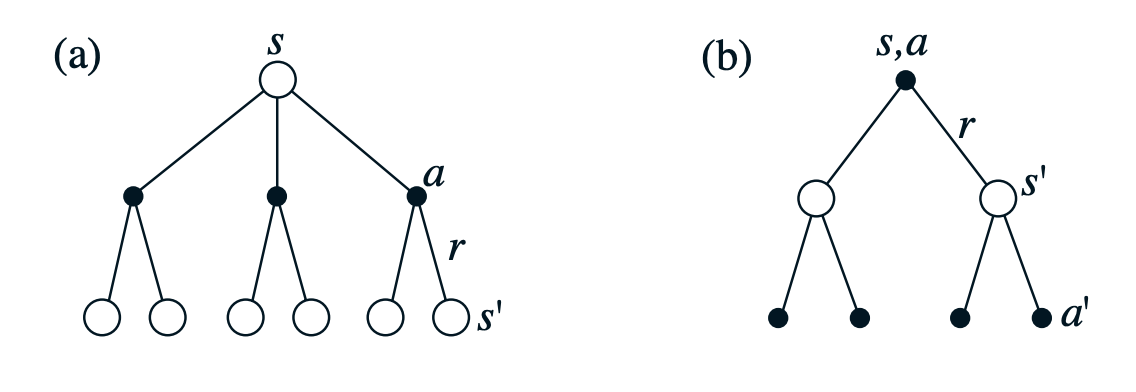
\includegraphics[width=\textwidth]{/chapter3_2}
	\caption{Backup diagrams for \(v_\pi\) and \(q_\pi\)}
	\label{fig:backup}
\end{figure}

\subsection{Optimal Policies and Value Functions}
\begin{itemize}
\item A policy \(\pi '\) is defined as better than policy pi if its expected return is higher for all states.
\item There is always \textit{at least} one policy that is better than or equal to all other policies - this is the \textit{optimal policy}.
\item Optimal policies are denoted \(\pi_*\)
\item Optimal state-value functions are denoted \(v_*\)
\item Optimal action-value functions are denoted \(q_*\)
\item We can write \(q_*\) in terms of \(v_*\):
\end{itemize}

\begin{equation}
q_*(s,a) = \mathbb{E} \left[R_{t+1} + \gamma v_*(S_{t+1}) | S_t = s, A_t = a \right]
\end{equation}

We can adapt the Bellman equation to achieve the Bellman optimality equation, which takes two forms. Firstly for \(v_*\):
\begin{equation}
v_*(s) = \max_{a \in \mathcal{A}(s)} \sum_{s',r} p(s', r | s, a) \left[r + \gamma v_*(s')\right]
\end{equation}
and secondly for \(q_*\):
\begin{equation}
q_*(s) = \sum_{s',r} p(s', r | s, a) \left[r + \gamma \max_{a'} q_*(s', a') \right]
\end{equation}

\begin{itemize}
\item Using \(v_*\) the optimal expected long term return is turned into a quantity that is immediately available for each state. Hence a one-step-ahead search, acting greedily, yield the optimal long-term actions.
\item Fully solving the Bellman optimality equations can be hugely expensive, especially if the number of states is huge, as is the case with most interesting problems.
\item Solving the Bellman optimality equation is akin to exhaustive search. We play out \textit{every} possible scenario until the terminal state and collect their expected reward. Our policy then defines the action that maximises this expected reward. 
\item In the continuous case the Bellman optimality equation is unsolvable as the recursion on the next state's value function would never end.
\end{itemize}

\subsection{Optimality and Approximation}
\begin{itemize}
	\item We must approximate because calculation of optimality is too expensive.
	\item A nice way of doing this is allowing the agent to make sub-optimal decisions in scenarios it has low probability of encountering. This is a trade off for being optimal in situations that occur frequently.
\end{itemize}

\subsection{Key Takeaways}
\begin{itemize}
\item We summarise our goal for the agent as a \textit{reward}; its objective is to maximise the cumulative sum of future rewards
\item For episodic tasks, returns terminate (and are backpropogated) when the episode ends. For the continuous control case, returns are discounted so they do not run to infinity. 
\item A state signal that succeeds in retaining all relevant information about the past is \textit{Markov}. 
\item Markov Decision Processes (MDPs) are the mathematically idealised version of the RL problem. They have system dynamics: $p(s', r | s, a) = Pr \{R_{r+1} = r, S_{t+1} = s' | S_t, A_t\}$
\item Policies are a (probabilistic) mapping from states to actions.
\item Value functions estimate how good it is for an agent to be in a state ($v_\pi$) or to take an action from a state ($q_\pi$). They are always defined w.r.t policies as the value of a state depends on the policy one takes in that state. Value functions are the \textit{expected cumulative sum of future rewards} from a state or state-action pair.
\item Knowing our policy and system dynamics, we can define the state value function is defined by the Bellman equation: $v_\pi(s) = \sum_{a} \pi(a|s) \sum_{s',r} p(s', r | s, a) \left[r + \gamma v_\pi(s')\right]$
\item An optimal policy ($\pi_*$) is the policy that maximises expected cumulative reward from all states. From the optimal policy we can derive the optimal value functions $q_*$ and $v_*$.
\end{itemize}











\section{Dynamic Programming}
Dynamic Programming (DP) refers to the collection of algorithms that can be used to compute optimal policies given a perfect model of the environment as an MDP. DP can rarely be used in practice because of their great cost, but are nonetheless important theoretically as all other approaches to computing the value function are, in effect, approximations of DP. DP algorithms are obtained by turning the Bellman equations into assignments, that is, into update rules for improving approximations of the desired value functions.

\subsection{Policy Evaluation (Prediction)}
We know from Chapter 3 that the value function can be represented as follows:
\begin{equation}
v_\pi(s) = \sum_{a} \pi(a|s) \sum_{s',r} p(s', r | s, a) \left[r + \gamma v_\pi(s')\right]
\end{equation}

If the dynamics are known perfectly, this becomes a system of $|\mathcal{S}|$ simultaneous linear equations in $|\mathcal{S}|$ unknowns, where the unknowns are $v_\pi(s), s \in \mathcal{S}$. If we consider an iterative sequence of value function approximations $v_0, v_1, v_2, \ldots$, with initial approximation $v_0$ chosen arbitrarily e.g. $v_k(s) = 0 \:  \forall s$ (ensuring terminal state = 0). We can update it using the Bellman equation:

\begin{equation}
v_{k+1}(s) = \sum_{a} \pi(a|s) \sum_{s',r} p(s', r | s, a) \left[r + \gamma v_k(s')\right]
\end{equation}

Eventually this update will converge when $v_k = v_\pi$ after infinite sweeps of the state-space, the value function for our policy. This algorithm is called \textit{iterative policy evaluation}. We call this update an \textit{expected update} because it is based on the expectation over all possible next states, rather than a sample of reward/value from the next state. We think of the updates occurring through \textit{sweeps} of state space.

\subsection{Policy Improvement}

We can obtain a value function for an arbitrary policy $\pi$ as per the policy evaluation algorithm discussed above. We may then want to know if there is a policy $\pi'$ that is better than our current policy. A way of evaluating this is by taking a new action $a$ in state $s$ that is not in our current policy, running our policy thereafter and seeing how the value function changes. Formally that looks like:
\begin{equation}
q_\pi(s, a) = \sum_{s',r} p(s', r | s, a) \left[r + \gamma v_\pi(s')\right]
\end{equation}

Note the mixing of action-value and state-value functions. If taking this new action in state $s$ produces a value function that is greater than or equal to the previous value function for all states then we say the policy $\pi'$ is an improvement over $\pi$:
\begin{equation}
v_{\pi'}(s) \geq v_\pi \forall s \in \mathcal{S}
\end{equation}

This is known as the \textit{policy improvement theorem}. Critically, the value function must be greater than the previous value function for all states. One way of choosing new actions for policy improvement is by acting greedily w.r.t the value function. Acting greedily will always produce a new policy $\pi' \geq \pi$, but it is not necessarily the optimal policy immediately.

\subsection{Policy Iteration}
By flipping between policy evaluation and improvement we can achieve a sequence of monotonically increasing policies and value functions. The algorithm is roughly:
\begin{enumerate}
\item Evaluate policy \(\pi\) to obtain value function \(V_\pi\)
\item Improve policy \(\pi\) by acting greedily with respect to \(V_\pi\) to obtain new policy \(\pi'\)
\item Evaluate new policy \(\pi'\) to obtain new value function \(V_{\pi'}\)
\item Repeat until new policy is no longer better than the old policy, at which point we have obtained the optimal policy. (Only for finite MDPs)
\end{enumerate}
This process can be illustrated as:
\begin{figure}[h!]
	\centering
	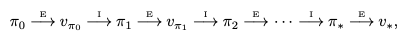
\includegraphics[width=\textwidth]{/chapter4_1}
	\caption{Iterative policy evaluation and improvement}
	\label{fig:policy evaluation}
\end{figure}

\subsection{Value Iteration}
Above, we discussed policy iteration which requires full policy evaluation at each iteration step, an often expensive process which (formally) requires infinite sweeps of the state space to approach the true value function. In value iteration, the policy evaluation is stopped after one visit to each $s \in \mathcal{S}$, or one \textit{sweep} of the state space. Value iteration is achieved by turning the Bellman optimality equation into an update rule:

\begin{equation}
v_{k+1}(s) = \argmax_a \sum_{s',r} p(s', r |s, a)\left[r + \gamma v_k(s')\right]
\end{equation}

for all $s \in \mathcal{S}$. Value iteration effectively combines, in each of its sweeps, one sweep of policy evaluation and one sweep of policy improvement. 

\subsection{Asynchronous Dynamic Programming}
Each of the above methods has required full sweeps of the state space to first evaluate a policy then improve it. Asynchronous dynamic programming does not require us to evaluate the entire state space each sweep. Instead, we can perform in place updates to our value function as they are experienced, focusing only on the most relevant states to our problem initially, then working to less relevant states elsewhere. This can mean that our agent can learn to act well more quickly and save optimality for later.

\subsection{Generalised Policy Iteration}
\begin{figure}[h!]
	\centering
	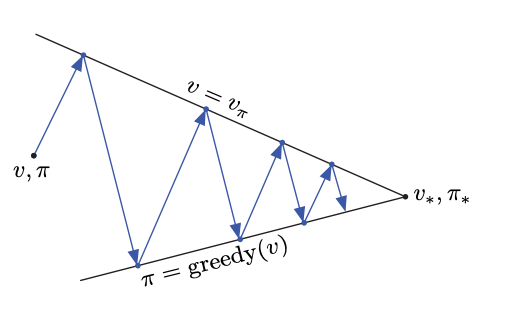
\includegraphics[width=0.5\textwidth]{/chapter4_2}
	\caption{Generalised policy iteration leading to optimality}
	\label{fig:gpi}
\end{figure}

Generalised Policy Iteration is the process of letting policy evaluation and policy improvement interact, independent of granularity. That is to say, improvement/evaluation can be performed by doing complete sweeps of the state space, or it can be performed after every visit to a state (as is the case with value iteration). The level of granularity is independent of our final outcome: convergence to the optimal policy and optimal value function. This process can be illustrated as two convergening lines - Figure \ref{fig:gpi}. We can see that policy improvement and policy evaluation work both in opposition and in cooperation - each time we act greedily we get further away from our true value function; and each time we evaluate our value function our policy is likely no longer greedy. 

\subsection{Key Takeaways}
\begin{itemize}
	\item \textit{Policy evaluation} is the iterative computation of a value function for a given policy. The value function is only truly evaluated in the limit.
	\item \textit{Policy improvement} is the computation of an improved policy given the value function for an existing policy.
	\item By combining the above we achieve \textit{Policy Iteration} and by performing each directly on the value function at each visit to a state we achieve \textit{Value Iteration} - both of which can be used to obtain optimal value functions and policies given complete knowledge of a finite Markov Decision Process.
	\item \textit{Generalised Policy Iteration} is the process of performing policy evaluation and improvement regardless of granularity - leading to convergence to the optimal value functions.
	\item DP methods operate in sweeps through the state space performing an \textit{expected update} operation at each state. These updates are based on expected values at all subsequent states and their probabilities of occurring. In general this idea is known as \textit{bootstrapping}, many RL methods bootstrap to update current beliefs from past beliefs.
\end{itemize}

\section{Monte Carlo Methods}
If we do not have knowledge of the transition probabilities (model of the environment) then we must learn directly from experience. To do so, we use Monte Carlo methods. Monte carlo methods are most effective in episodic tasks where there is a terminal state and the value of the states visited en route to the terminal state can be updated based on the reward received at the terminal state. We use general policy iteration as outlined in chapter 4, but this time instead of \textit{computing} the value function we \textit{learn} it from samples. We first consider the prediction problem to obtain $v_\pi$ and/or \textbf{$q_\pi$} for a fixed policy, then we look to improve using policy improvement, then we use it for control.  

\subsection{Monte Carlo Policy Prediction}
\begin{itemize}
\item Recall that the value of a state is the expected discounted future reward from that state. One way of estimating that value is by observing the rewards obtained after visiting the state, we would expect that in the limit this would converge toward the true value.
\item We can therefore run a policy in an environment for an episode. When the episode ends, we receive a reward and we assign that reward to each of the states visited en route to the terminal state. 
\item Where DP algorithms perform one-step predictions to \textit{every} possible next state; monte-carlo methods only sample one trajectory/episode. This can be summarised in a new backup diagram as follows:
\begin{figure}[h!]
	\centering
	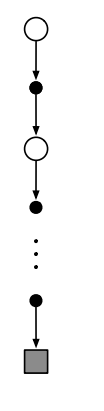
\includegraphics[width=0.1\textwidth]{/chapter5_1}
	\caption{Monte carlo backup diagram for one episode}
	\label{fig:monte carlo backup}
\end{figure}

\item Importantly, monte carlo methods do not bootstrap in the same way DP methods do. They take the reward at the end of an episode, rather than estimated reward based on the value of the next state.
\item Because of the lack of bootstrapping, this expense of estimating the value of one state is independent of the number of states, unlike DP. A significant advantage, in addition to the other advantages of being able to learn from experience without a model or from simulated experience. 
\end{itemize}

\subsection{Monte Carlo Estimation of Action Values}
\begin{itemize}
\item With a model we only need to estimate the state value function \(v\) as, paired with our model, we can evaluate the rewards and next states for each of our actions and pick the best one.
\item With model free methods we need to estimate the state-action value function \(q\) as we must explicitly estimate the value of each action in order for the values to be useful in suggesting a policy. (If we only have the values of states, and don't know how states are linked through a model, then selecting the optimal action is impossible)
\item One serious complication arises when we do not visit every state, as can be the case if our policy is deterministic. If we do not visit states then we do not observe returns from these states and cannot estimate their value. We therefore need to \textit{maintain exploration} of the state space. One way of doing so is stochastically selected a state-action pair to start an episode, giving every state-action pair a non-zero probability of being selected. In this case, we are said to be utilising \textit{exploring starts}.
\item Exploring starts falls down when learning from real experience because we cannot guarantee that we start in a new state-action pair in the real world. 
\item An alternative approach is to use stochastic policies that have non-zero probability of selecting each state-action pair.
\end{itemize}


\subsection{Monte Carlo Control}
\begin{itemize}
\item Much like we did with value iteration, we do not need to fully evaluate the value function for a given policy in monte carlo control. Instead we can merely \textit{move} the value toward the correct value and then switch to policy improvement thereafter. It is natural to do this episodically i.e. evaluate the policy using one episode of experience, then act greedily w.r.t the previous value function to improve the policy in the next episode.
\item If we use a deterministic policy for control, we must use exploring starts to ensure sufficient exploration. This creates the \textit{Monte Carlo ES} algorithm.
\end{itemize}

\subsection{Monte Carlo Control without Exploring Starts}
\begin{itemize}
\item To avoid having to use exploring starts we can use either \textit{on-policy} or \textit{off-policy} methods. The only way to ensure we visit everything is to visit them directly.
\item On-policy methods attempt to improve or evaluate or improve the policy that is making decisions.
\item On-policy control methods are generally \textit{soft} meaning that they assign non-zero probability to each possible action in a state e.g. e-greedy policies.
\item We take actions in the environment using e-greedy policy, after each episode we back propagate the rewards to obtain the value function for our e-greedy policy. Then we perform policy improvement by updating our policy to take the \textbf{new} greedy reward in each state. Note: based on our new value function, the new greedy action may have changed in some states. Then we perform policy evaluation using our new e-greedy policy and repeat (as per generalised policy iteration).
\item The idea of on-policy Monte Carlo control is still that of GPI. We use first visit MC methods to estimate the action-value function i.e. to do policy evaluation, but we cannot then make improve our policy merely by acting greedily w.r.t our value function because that would prevent further exploration of non-greedy actions. We must maintain exploration and so improve the $\epsilon$-greedy version of our policy. That is to say, when we find the greedy action (the action that maximises our reward for our given value function) we assign it probability $1 - \epsilon + \frac{\epsilon}{\mathcal{A}(S_t)}$ of being selected so that the policy remains stochastic.
\item Note: doing the above will only find us the best policy amongst the $\epsilon$-soft policies, which may not be the optimal policy for the environment, but it does allow us to remove the need for exploratory starts.
\end{itemize}

\subsection{Off-policy Prediction via Importance Sampling}
We face a dilemma when learning control: we want to find the optimal policy, but we can only find the optimal policy by acting suboptimally to explore sufficient actions. What we saw with on-policy learning was a compromise - it learns action values not for the optimal policy but for a near-optimal policy that still explores. An alternative is off-policy control where we have two policies: one used to generate the data (behaviour policy) and one that is learned for control (target policy). This is called \textit{off policy learning}.

\begin{itemize}
\item Off-policy learning methods are powerful and more general than on-policy methods (on-policy methods being a special case of off-policy where target and behaviour policies are the same). They can be used to learn from data generated by a conventional non-learning controller or from a human expert.
\item If we consider an example of finding target policy $\pi$ using episodes collected through a behaviour policy $b$, we require that every action in $\pi$ must also be taken, at least occasionally, by $b$ i.e. $\pi(a|s) > 0$ implies $b(a|s) > 0$. This is called the assumption of \textit{\textbf{coverage}}. 
\item Almost all off-policy methods utilize \textit{importance sampling}, a general technique for estimating expected values under one distribution given samples from another. Given a starting state $S_t$, the probability of the subsequent state-action trajectory occuring under any policy $\pi$ is:

\begin{equation}
	\prod_{k=t}^{T-1} \pi(A_k|S_k)p(S_{k+1}|S_k, A_k)
\end{equation}

where $p$ is the state transition probability function. We can then obtain the relative probability of the trajectory under the target and behaviour policies (the importance sampling ratio) as:

\begin{equation} \label{eq: importance sampling ratio}
p_{t:T-1} = \frac{\prod_{k=t}^{T-1} \pi(A_k|S_k)p(S_{k+1}|S_k, A_k)}{\prod_{k=t}^{T-1} b(A_k|S_k)p(S_{k+1}|S_k, A_k)} = \prod_{k=t}^{T-1} \frac{\pi(A_k|S_k)}{b(A_k|S_k)}
\end{equation}

We see here that the state transition probability function helpfully cancels.

\item We want to estimate the expected returns under the target policy but we only have returns from the behaviour policy. To address this we simply multiply expected returns from the behaviour policy by the importance sampling ratio to get the value function for our target policy.

\begin{equation}
\mathbb{E} \left[p_{t:T-1} G_t | S_t = s\right] = v_\pi(s)
\end{equation}

\item Note: importance sampling ratios are only non-zero for episodes where the target-policy has non-zero probability of acting \textit{exactly} like the behaviour policy $b$. So, if the behaviour policy takes 10 steps in an episode, each of these 10 steps have to have been \textit{possible} by the target policy, else $\pi(a|s) = 0$ and $\rho_{t:T-1} = 0$.

\end{itemize}

\subsection{Incremental Implementation}
We perform monte carlo policy evaluation (prediction) incrementally in the same way as was done in Chapter 2 for the bandit problem. Generally incremental implementation follows this formula:

\begin{equation}
New Estimate \leftarrow Old Estimate + Step Size \left[Observation - Old Estimate \right]
\end{equation}

With on-policy monte carlo methods, this update is performed exactly after each episode for each visit to a state given the observed rewards, with off-policy methods the update is slightly more complex. With ordinary importance sampling, the step size is $1/n$ where $n$ is the number of visits to that state, and so acts as an average of the scaled returns. For weighted importance sampling, we have to form a weighted average of the returns which requires us to keep track of the weights. If the weight takes the form $W_i = \rho_{t:T(t)-1}$ then our update rule is:

\begin{equation} \label{incremental V}
V_{n+1} = V_n + \frac{W_n}{C_n}\left[G_n - V_n\right]
\end{equation}
where,
\begin{equation}
C_{n+1} = C_n + W_{n+1}
\end{equation}
with $C_0 = 0$. This allows us to keep tracking of the corrected weighted average term for each update as they are made. Note here that the weighted average gives more weight to updates based on common trajectories from $b$ in $\pi$ that we have some more often.

\subsection{Off-policy Monte Carlo Control}
Using incremental implementation (updates to the value function) and importance sampling we can now discuss \textit{off-policy monte carlo control}–the algorithm for obtaining optimal policy $\pi_*$ by using rewards obtained through behaviour policy $b$. This works in much the same way as in previous sections; $b$ must be $\epsilon$-soft to ensure the entire state space is explored in the limit; updates are only made to our estimate for $q_\pi$, $Q$, if the sequence of states an actions produced by $b$ could have been produced by $\pi$. This algorithm is also based on GPI: we update our estimate of $Q$ using Equation \ref*{incremental V}, then update $\pi$ by acting greedily w.r.t to our value function. If this policy improvement changes our policy such that the trajectory we are in from $b$ no longer obeys our policy, then we exit the episode and start again. The full algorithm is shown in \ref*{fig:Off-policy monte carlo control}.

\begin{figure}[h!]
	\centering
	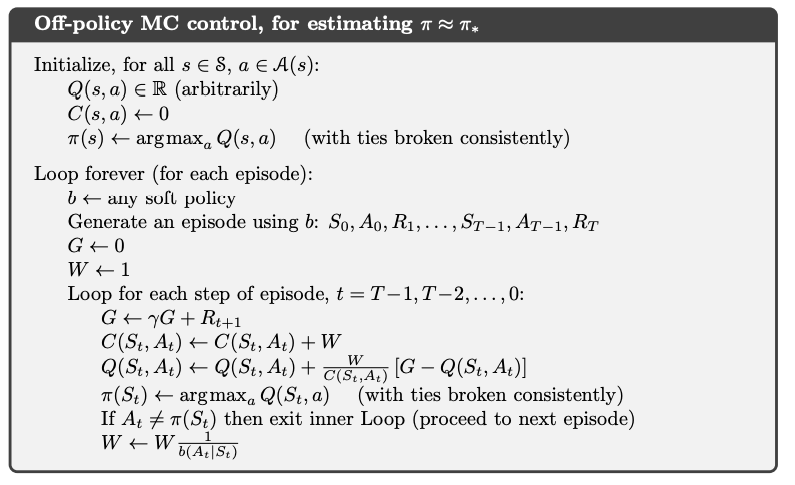
\includegraphics[width=0.8\textwidth]{/chapter5_3}
	\caption{Off-policy monte carlo control}
	\label{fig:Off-policy monte carlo control}
\end{figure}

\subsection{Key Takeaways}
\begin{itemize}
\item In the absence of a model of the environment, monte carlo methods allow us to evaluate and improve our value function based on \textit{experience}
\item We roll-out trajectories to terminal states, and back-propagate the rewards to the states visited en-route in several ways
\item Monte carlo methods use GPI (see chapter 4) in much the same way dynamic programming does. We evaluate our policy, then improve by acting greedily w.r.t our new value function until we converge on the optimal value function and policy.
\item Differences with dynamic programming methods: 1) They do not require a model of the environment as they learn directly from experience, and 2) They do not bootstrap i.e. the value function estimates are an average of all real returns accumulated after visiting the state.
\item Maintaining sufficient exploration is crucial with monte carlo methods; if our policy is deterministic we will likely not explore the full states space during our roll-outs. To deal with this we have several options: 1) Start every episode randomly with uniform probability such that we make sure we start at each possible state–called \textit{exploring starts}, unrealistic in the real world as we can't make a robot restart from all possible states. Or 2) Use $\epsilon$-soft policies that have a non-zero probability of selecting all possible states. The downside of doing this is that we will converge on the optimal $\epsilon$-soft, which is not necessarily the optimal policy for the environment, because it needs to learn how account for its own randomness. This is the price we pay for exploration.
\item Monte carlo methods can either be \textit{on-policy} or \textit{off-policy}.
\item On-policy methods use the same policy to collect data as is evaluated and improved. This suffers the downsides outlined above.
\item Off-policy methods have two policies, one that collects the data called the \textit{behaviour policy} $b$ and the other which we look to improve called the target policy $\pi$. We find trajectories from the behaviour policy that line up with our target policy, that is to say, that could have been produced by our target policy. This process only works if the behaviour policy has non-zero probability of selecting each of the actions in the target policy, aka \textit{coverage} of the target policy. The agent explores, but learns a deterministic optimal policy offline that may be unrelated to the behaviour policy used to collect the experience.
\item Based on rewards observed by running the behaviour policy, we update our value function using \textit{importance sampling}, which measures, if effect, how likely the observed behaviour would have been given our target policy. For example, the target policy may take 1 of 4 actions with equal probability in each state. If we observe two timesteps from our beaviour policy, then our probability of selecting the actions taken by the behaviour policy would be $0.25 \times 0.25$. 
\item We weight each return using the \textit{importance sampling ratio}, a measure of how likely we were to produce the roll-out using the target policy compared to how likely we were to produce the roll-out using the behaviour policy. 
\item Importance sampling can be \textit{ordinary} i.e. an average of the returns observed from a state or \textit{weighted} where trajectories viewed more often, or with a higher importance sampling ratio give the value update more weight.

\end{itemize}
\section{Temporal-Difference Learning}

TD learning is novel to RL. It is a hybrid that lies between monte carlo and dynamic programming methods. As with those, TD learning uses GPI; control (policy improvement) works in much the same way, it is in the prediction of the value function (policy evaluation) where the distinctions lie.

\subsection{TD Prediction}
Monte carlo methods wait until the end of the episode before back-propagating the return to the states visited en-route. The simplest TD method (TD(0)) does not wait until the end of the episode, in fact, it updates its estimate of the value function $V(s)$ based on the instantaneous reward as follows:
\begin{equation} \label{eq: td}
V(S_t) \leftarrow V(S_t) + \alpha \left[R_{t+1} + \gamma V(S_{t+1}) - V(S_t)\right]
\end{equation}

Note here, that TD(0) \textit{bootstraps} in much the same way DP methods do i.e. it bases it's estimate of $V(s)$ on the value of the next state $V(s')$. TD methods therefore take both sampling from monte carlo, and bootstrapping from DP. The TD(0) backup diagram is shown in Figure \ref{fig:td(0)}.

\begin{figure}[h!]
	\centering
	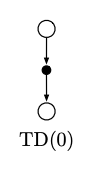
\includegraphics[width=0.2\textwidth]{/chapter6_1}
	\caption{Backup diagram for TD(0)}
	\label{fig:td(0)}
\end{figure}

The quantity in the brackets of equation \ref{eq: td} is known as the \textit{TD error}. Formally this is expressed as:
\begin{equation}
\delta_t = R_{t+1} + \gamma V(S_{t+1}) - V(S_t)
\end{equation}

\begin{figure}[h!]
	\centering
	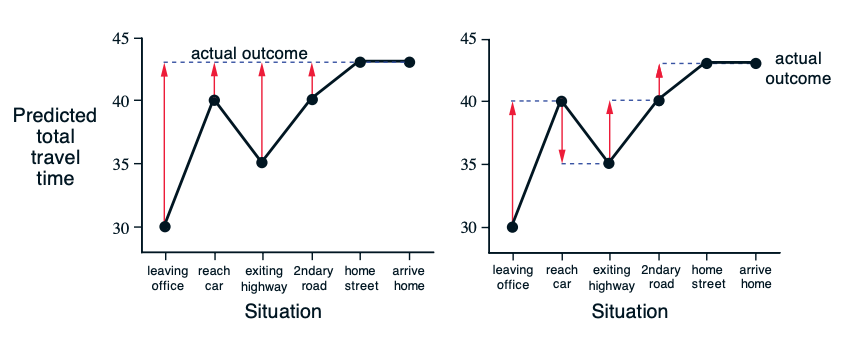
\includegraphics[width=\textwidth]{/chapter6_2}
	\caption{Monte carlo updates (left) and TD-updates (right) to the value function associated with a daily commute}
	\label{fig:td vs. mc}
\end{figure}

In Figure \ref{fig:td vs. mc} we see the differences between monte carlo and TD updates to the value function. In the case of monte carlo, we would need to wait until we arrived home before we could update our predictions for journey length. With TD learning, we can adjust these estimates on the fly based on the error in our predictions en-route. We see here that the adjustment we make changes at each timestep depending on the difference between predictions, that is to say, the update is proportional to the \textit{temporal differences} between our predictions across timesteps.

\subsection{Advantages of TD Prediction Methods}
\begin{itemize}
\item TD methods generally converge faster than MC methods, although this has not been formally proven.
\item TD methods do converge on the value function with a sufficiently small step size parameter, or with a decreasing stepsize.
\item They are extremely useful for continuing tasks that cannot be broken down in episodes as required by MC methods.
\end{itemize}

\subsection{Optimality of TD(0)}
If we only have a finite number of episodes or training data to learn from we can update our value function in \textit{batches}. We repeatedly play the same data, and update our value function by the sum of each of the increments for each state at the end of the batch.

TD batching and Monte Carlo batching converge often on two different estimates of the value function. The monte carlo batch estimate can only judge based on observed rewards from a state, but TD batching can make estimates based on later states using bootstrapping. Example 6.4 (\textit{You are the predictor}) on pg 127 explains this excellently. The monte carlo estimate will converge on the correct estimate of the value function produced by the training data, but TD methods will generalise better to future rewards because they preserve the transition from state-to-state in the TD update, and thus bootstrap better from values of other states.

In general batch MC methods always minimise the mean squared error or the training set whereas TD(0) finds the estimates that would be exactly correct for the maximum-likelihood model of the Markov process. This is called the \textit{certainty equivalence estimate} because it is equivalent to assuming that the estimate of the underlying process was known with certainty rather than being approximated.

\subsection{Sarsa: On-policy TD Control}
We'll now look at using TD prediction methods for control. We'll follow, as before, the framework of Generalised Policy Iteration (GPI), only this time using TD methods for predicting the value function.
For on-policy control, we wish to learn the state-action value function for our policy $q_\pi(s,a)$ and all states $s$ and actions $a$. We amend the TD update formula provided in Equation \ref{eq: td} to account for state-action values:
\begin{equation}
Q(S_t, A_t) \leftarrow Q(S_t, A_t) + \alpha \left[R_{t+1} + \gamma Q(S_{t+1}, A_{t+1}) - Q(S_t, A_t) \right]
\end{equation}

This produces a quintuple of events: $(S_t, A_t, R_{t+1}, S_{t+1}, A_{t+1})$ giving rise to the name SARSA. As with other on-policy control algorithms, we update our policy to be greedy w.r.t our ever-changing value function.

\subsection{Q-learning: Off-policy TD Control}
Q-learning, much like SARSA, makes 1-step updates to the value function, but does so in subtly different ways. SARSA is on-policy, meaning it learns the optimal version of the policy used for collecting data i.e. an $\epsilon$-greedy policy to ensure the state-space is covered. This limits its performance as it needs to account for the stochasticity of exploration with probability $\epsilon$. Q-learning, on the other hand, is off-policy and directly predicts the optimal value function $q_*$ whilst using an $\epsilon$-greedy policy for exploration. Updates to the state-action value function are performed as follows:
\begin{equation}
Q(S_t, A_t) \leftarrow Q(S_t, A_t) + \alpha \left[R_{t+1} + \gamma \max_{a} Q(S_{t+1}, a) - Q(S_t, A_t) \right]
\end{equation}

We observe that the max action selection at next state $S_{t+1}$ means we are no longer following an $\epsilon$-greedy policy for our updates. Q-learning has been shown to converge to $q_*$ with probability 1.

\subsection{Expected Sarsa}
Instead of updating our value function with the value maximising action at $S_{t+1}$ (as is the case with Q-learning) or with the action prescribes by our $\epsilon$-greedy policy (as is the case with SARSA), we could make updates based on the \textit{expected value} of $Q$ at $S_{t+1}$. This is the premise of expected sarsa. Doing so reduces the variance induced by selecting random actions according to an $\epsilon$-greedy policy. It's update is described by:
\begin{align}
Q(S_t, A_t) &\leftarrow Q(S_t, A_t) + \alpha \left[R_{t+1} + \gamma \mathbb{E}_\pi Q(S_{t+1}, A_{t+1} | S_{t+1}) - Q(S_t, A_t) \right] \\
&\leftarrow Q(S_t, A_t) + \alpha \left[R_{t+1} + \gamma \sum_{a} \pi(a | S_{t+1}) Q(S_{t+1}, a) - Q(S_t, A_t) \right] \\
\end{align}

We can adapt expected SARSA to be off-policy by making our target policy $\pi$ greedy, in which case expected SARSA becomes Q-learning. It is therefore seen as a generalisation of Q-learning that reliably improves over SARSA.

\subsection{Maximization Bias and Double Learning}
Many of the algorithms discussed so far in these notes use a maximisation operator to select actions - either $\epsilon$-greedy or greedy action selection. Doing so means we implicitly favour positive numbers. If the true values of state action pairs are all zero i.e. $Q(S,A) = 0 \forall \; s, a$, then, at some stage in learning, we are likely to have distributed value estimates around 0. Our maximisation operator will select the postive value estimates, despite the latent values being 0. Thus we bias positive values, a so-called \textit{maximisation bias}.

We can counter this by learning two estimates of the value function $Q_1$ and $Q_2$. We use one to select actions from a state e.g. $A^* = \argmax_a Q_1(a)$ and then use the other to provide an estimate of its value $Q_2(A^*) = Q_2(\argmax_a Q_1(a))$. This estimate will be unbiased in the sense that $\mathbb{E}\left[Q_2(A^*)\right] = q(A^*)$. 

\subsection{Games, Afterstates, and Other Special Cases}
Much of the theory in this book revolves around action-value functions, where the value of an action in a given state is quantified \textbf{before} the action is taken. In some settings, it is expedient to quantify value functions after an action, as many actions may lead to the same state afterward. This is the case for the game tic-tac-toe, as described in the book. In certain circumstances, it can be beneficial to amend value functions to accommodate afterstates if this property is shown.

\subsection{Key Takeaways}
\begin{itemize}
	\item TD methods update value functions en-route to episode termination, rather than waiting to the end of the episode like Monte Carlo methods. Updates to the value function are made in proportion to the \textit{temporal differences} between value function estimates.
	\item TD methods bootstrap off of value function estimates elsewhere in the state space, and consequently generalise to new data better than MC methods, which cannot make predictions outside of the observed training data.
	\item TD methods continue to follow the framework of Generalised Policy Iteration (GPI) as discussed in previous chapters.
	\item SARSA is the eminent on-policy TD method, but is limited in that in can only ever learn the optimal $\epsilon$-soft behaviour policy.
	\item Q-learning is the eminent off-policy TD method, that will learn the optimal policy $\pi_*$ with probability 1.
	\item Expected SARSA makes updates based on the expected value of the next state given a policy, reducing the variance induced by an $\epsilon$-soft behaviour policy, performing better than SARSA given the same experience.
	\item The postive bias of action selection via maximisation can be mitigated by double learning methods.
\end{itemize}














\documentclass[a4paper, oneside, 11pt]{article}
\usepackage[margin=2.5cm]{geometry}
\usepackage{amssymb}
\usepackage{amsmath}
\usepackage{graphicx}
\usepackage{bm}
\usepackage{mathtools}
\usepackage{setspace}
\usepackage{dsfont}
\usepackage{xcolor}
\usepackage{upquote}
\usepackage[utf8]{inputenc}
\usepackage[colorlinks=true, linkcolor=black, urlcolor=blue, citecolor=black]{hyperref}

\usepackage[shortlabels]{enumitem}

\setlength{\parindent}{0cm}

\newcommand\Rule{\noindent\makebox[\textwidth]{\rule{\textwidth}{0.5pt}}}

\newcommand\argmax{\operatorname*{argmax}}
\newcommand\argmin{\operatorname*{argmin}}

\renewcommand{\vec}[1]{\boldsymbol{#1}}

\newcommand{\R}{\mathbb{R}}
\newcommand\Epi{\mathbb{E}_{\pi}}
\renewcommand\P{\mathbb{P}}
\newcommand\E{\mathbb{E}}
\newcommand{\VE}{\overline{\mathrm{VE}}}

\renewcommand{\S}{\mathcal{S}}
\newcommand{\A}{\mathcal{A}}
\newcommand{\grad}{\nabla}
\renewcommand{\d}{\mathrm{d}}


\renewcommand{\familydefault}{\sfdefault}


\newcommand\RepoAddress{https://github.com/brynhayder/reinforcement_learning_an_introduction}
\newcommand\RepoName{github.com/brynhayder/reinforcement\_learning\_an\_introduction}

\newcommand\ProjectDir{/Users/Bryn/Programming/remote/ReinforcementLearningAnIntroduction}
\newcommand\NotesImages{\ProjectDir/data/notes_images}
\newcommand\ExerciseOutput{\ProjectDir/data/exercise_output}

\newcommand\ProgrammingExercise{This is a programming exercise. For the relevant code please see \href{\RepoAddress{}}{the repo}.}



\begin{document}
    \section{$n$-step Bootstrapping}
$n$-step methods allow us to observe multiple time-steps of returns before updating a state with the observed data and a bootstrapped estimate of the value of the $n$th succeeding state.

\subsection{$n$-step TD Prediction}
Define the $n$-step return
\begin{equation}
    G_{t:t+n} \doteq \sum_{i=t}^{t+n-1}\gamma^{i-t}R_{i+1} + \gamma^n V_{t+n-1}(S_{t+n})
\end{equation}
where $n \geq 1$, $0 \leq t < T - n$ and $V_i$ is the estimated state-value function as of time $i$. If $t + n > T$ then $G_{t+n} \equiv G_t$, the standard return. The $n$-step return is the target for \emph{$n$-step TD} methods, note that $n-1$ rewards are observed and the succeeding value is bootstrapped with the latest estimate of the value function. The corresponding update for state-values is
\begin{equation}
    V_{t+n}(S_t) = V_{t+n - 1}(S_t) + \alpha [G_{t:t+n} - V_{t+n-1}(S_{t})]  \quad\quad 0 \leq t < T.
\end{equation}
Note that Monte-Carlo can be thought of as TD($\infty$)Pseudocode for $n$-step TD is given in the box below.\\

\includegraphics[width=\textwidth]{\NotesImages/n_step_td_state_values.png}\\

The $n$-step return obeys the \emph{error-reduction property}, and because of this $n$-step TD can be shown to converge to correct predictions (given a policy) under appropriate technical conditions. This property states that the $n$-step return is a better estimate than $V_{t+n-1}$ in the sense that the error on the worst prediction is always smaller
\begin{equation}
    \max_s \left|\Epi[G_{t:t+n}|S_t=s] - v_\pi(s)\right| \leq \gamma^n \max_s \left|V_{t+n-1}(s) - v_\pi(s)\right|
\end{equation}

\subsection{$n$-step Sarsa}
\subsubsection*{Sarsa}
We develop $n$-step methods for control. We generalise Sarsa to $n$-step Sarsa, or Sarsa($n$). This is done in much the same way as above, but with action-values as opposed to state-values. The $n$-step return in this case is defined as
\begin{equation}
    G_{t:t+n} \doteq \sum_{i=t}^{t+n-1}\gamma^{i-t}R_{i+1} + \gamma^n Q_{t+n-1}(S_{t+n}, A_{t+n})
\end{equation}
where $n \geq 1$, $0 \leq t < T - n$ and $Q_i$ is the estimated action-value function as of time $i$. If $t + n > T$ then $G_{t+n} \equiv G_t$, the standard return. The corresponding update is
\begin{equation}
    Q_{t+n}(S_t, A_t) = Q_{t+n-1}(S_t, A_t) + \alpha [G_{t:t+n} - Q_{t+n-1}(S_{t}, A_{t})]  \quad\quad 0 \leq t < T.
\end{equation}

\subsubsection*{Expected Sarsa}
We define $n$-step expected Sarsa similarly
\begin{equation}
    G_{t:t+n} \doteq \sum_{i=t}^{t+n-1}\gamma^{i-t}R_{i+1} + \gamma^n \bar{V}_{t+n-1}(S_{t+n})
\end{equation}
where $n \geq 1$, $0 \leq t < T - n$ and $\bar{V}_i$ is the \emph{expected approximate value} of state $s$
\begin{equation}
    \bar{V}_i(s) \doteq \sum_a \pi(a|s)Q_i(s, a).
\end{equation} 
As always, if $t + n > T$ then $G_{t+n} \equiv G_t$, the standard return. The corresponding update is formally the same as above\\


\includegraphics[width=\textwidth]{\NotesImages/n_step_sarsa.png}\\

\subsection{$n$-step Off-policy Learning}
We can learn with $n$-step methods off-policy using the importance sampling ratio (target policy $\pi$ and behaviour policy $b$)
\[
    \rho_{t:h} \doteq \prod_{k=t}^{\text{min}(h, T-1)}\frac{\pi(A_k|S_k)}{b(A_k|S_k)}.
\]
For state-values we have 
\[
    V_{t+n}(S_t) \doteq V_{t+n-1}(S_t) + \alpha \rho_{t:t+n-1}[G_{t:t+n} - V_{t+n-1}(S_t)]
\]
and for action-values we have
\[
    Q_{t+n}(S_t, A_t) = Q_{t+n-1}(S_t, A_t) + \alpha \rho_{t+1:t+n-1}[G_{t:t+n} - Q_{t+n-1}(S_t, A_t)]
\]
note that for action values the importance sampling ratio starts one time-step later, because we are attempting to discriminate between actions at time $t$.\\

\includegraphics[width=\textwidth]{\NotesImages/off_policy_n_step_sarsa.png}\\

\subsection{*Per-decision Methods with Control Variates}
We have the standard recursion relation for the $n$-step return
\[
    G_{t:h} = R_{t+1} + \gamma G_{t+1:h}.
\]
For an off-policy algorithm, one would be tempted to simply weight this target by the importance sampling ratio. This method, however, shrinks the estimated value functions when the importance sampling ratio is 0, hence increasing variance. We thus introduce the \emph{control-variate} $(1 - \rho_t)V_{h-1}(S_t)$, giving an off-policy update of 
\[
    G_{t:h} = \rho_t (R_{t+1} + \gamma G_{t+1:h}) + (1 - \rho_t)V_{h-1}(S_t)
\]
where $G_{h:h} = V_{h-1}(S_h)$. Note that the control-variate has expected value 0, since the factors are uncorrelated and the expected value of the importance sampling ratio is 1.\\

We can do a similar thing for action-values
\[
    G_{t:h} \doteq R_{t+1} + \gamma \rho_{t+1:h}\left( G_{t+1:h} - Q_{h-1}(S_{t+1}, A_{t+1}) \right) - \gamma \bar{V}_{h-1}(S_{t+1}),
\]
where once again the importance sampling ratio starts one time-step later.

\subsubsection*{Control Variates in General}
Suppose we want to estimate $\mu$ and assume we have an unbiased estimator for $\mu$ in $m$. Suppose we calculate another statistic $t$ such that $\mathbb{E}\left[t\right]=\tau$ is a known value. Then
\[
    m^\star = m + c\left(t-\tau\right)
\]
is also an unbiased estimator for $\mu$ for any $c$, with variance
\[
    \textrm{Var}\left(m^{\star}\right)=\textrm{Var}\left(m\right) + c^2\,\textrm{Var}\left(t\right) + 2c\,\textrm{Cov}\left(m,t\right).
\]

It is easy to see that taking

\[
    c = - \frac{\textrm{Cov}\left(m,t\right)}{\textrm{Var}\left(t\right)}
\]
minimizes the variance of $m^{\star}$. With this choice

\begin{align}
\textrm{Var}(m^{\star}) & =\textrm{Var}(m) - \frac{\left[\textrm{Cov}(m,t)\right]^2}{\textrm{Var}(t)} \\
& = (1-\rho_{m,t}^2)\textrm{Var}(m)
\end{align}
where $\rho_{m,t}=\textrm{Corr}\left(m,t\right) $ is the Pearson correlation coefficient of $m$ and $t$. The greater the value of $|\rho_{m,t}|$, the greater the variance reduction achieved.

\subsection{Off-policy Learning Without Importance Sampling: The $n$-step Tree Backup Algorithm}
We introduce the $n$-step \emph{tree-backup algorithm} algorithm using the return
\begin{equation}
    G_{t:t+n} \doteq R_{t+1} + \gamma \sum_{a \neq A_{t+1}} \pi(a|S_{t+1})Q_{t+n-1}(S_{t+1}, a) + \gamma \pi(A_{t+1}|S_{t+1})G_{t+1:t+n}
\end{equation}
for $t < T-1$, $n > 1$ and with $G_{i:i} = 0$ and $G_{T-1:t+n} = R_T$. This algorithm updates $S_t$ with bootstrapped, probability weighted action-values of \emph{all} actions that were not taken all along the trajectory and recursively includes the rewards realised, weighted by the probability of their preceding actions under the policy. Pseudocode given below.\\

\includegraphics[width=\textwidth]{\NotesImages/n_step_tree_backup.png}\\
    
    
\subsection{*A Unifying Algorithm: $n$-step $Q(\sigma)$}
We introduce an algorithm which, at each time step, can choose to either take an action as a sample as in Sarsa or to take an expectation over all possible actions as in tree-backup. \\

Define a sequence $\sigma_t \in [0, 1]$ that at each time step chooses a proportion of sampling vs. expectation. This generalises Sarsa and tree-backup by allowing each update to be a linear combination of the two ideas. The corresponding return (off-policy) is 
\begin{align}
    G_{t:h} \doteq R_{t+1} &+ \gamma \left(\sigma_{t+1}\rho_{t+1}  (1- \sigma_{t+1})\pi(A_{t+1}\vert S_{t+1})\right) \left( G_{t+1:h} - Q_{h-1}(S_{t+1}, A_{t+1}) \right) \\ 
                           &+ \gamma \bar{V}_{h-1}(S_{t+1}),
\end{align}
for $t < h< T$, with $G_{h:h} \doteq Q_{h-1}(S_h, A_h)$ if $h<T$ and $G_{T-1:T} \doteq R_t$ if $h=T$. Pseudocode given below.\\

\includegraphics[width=\textwidth]{\NotesImages/off_policy_n_step_Q_sigma.png}\\

    
    
    
    
    
    
    
    
    
    


\end{document}
\documentclass[a4paper, oneside, 11pt]{article}
\usepackage[margin=2.5cm]{geometry}
\usepackage{amssymb}
\usepackage{amsmath}
\usepackage{graphicx}
\usepackage{bm}
\usepackage{mathtools}
\usepackage{setspace}
\usepackage{dsfont}
\usepackage{xcolor}
\usepackage{upquote}
\usepackage[utf8]{inputenc}
\usepackage[colorlinks=true, linkcolor=black, urlcolor=blue, citecolor=black]{hyperref}

\usepackage[shortlabels]{enumitem}

\setlength{\parindent}{0cm}

\newcommand\Rule{\noindent\makebox[\textwidth]{\rule{\textwidth}{0.5pt}}}

\newcommand\argmax{\operatorname*{argmax}}
\newcommand\argmin{\operatorname*{argmin}}

\renewcommand{\vec}[1]{\boldsymbol{#1}}

\newcommand{\R}{\mathbb{R}}
\newcommand\Epi{\mathbb{E}_{\pi}}
\renewcommand\P{\mathbb{P}}
\newcommand\E{\mathbb{E}}
\newcommand{\VE}{\overline{\mathrm{VE}}}

\renewcommand{\S}{\mathcal{S}}
\newcommand{\A}{\mathcal{A}}
\newcommand{\grad}{\nabla}
\renewcommand{\d}{\mathrm{d}}


\renewcommand{\familydefault}{\sfdefault}


\newcommand\RepoAddress{https://github.com/brynhayder/reinforcement_learning_an_introduction}
\newcommand\RepoName{github.com/brynhayder/reinforcement\_learning\_an\_introduction}

\newcommand\ProjectDir{/Users/Bryn/Programming/remote/ReinforcementLearningAnIntroduction}
\newcommand\NotesImages{\ProjectDir/data/notes_images}
\newcommand\ExerciseOutput{\ProjectDir/data/exercise_output}

\newcommand\ProgrammingExercise{This is a programming exercise. For the relevant code please see \href{\RepoAddress{}}{the repo}.}



\begin{document}
    \section{Planning and Learning with Tabular Methods}


\subsection{Models and Planning}
A \emph{model} of the environment is anything that an agent can use to predict how the environment will respond to its actions. A \emph{distribution model} is one that characterises the distribution of possible environmental changes, whereas a \emph{sample model} is one that produces sample behaviour. Distribution models are in some sense stronger, in that they can be used to produce samples of the behaviour of the environment, but it is often easier to reproduce sample responses than to model the response distribution.\\

Models can be used to simulate the environment and hence simulate experience. We use the term \emph{planning} to refer to a computational process that uses a model for improving a policy. The kind of planning that we consider here falls under the name \emph{state-space planning}, since it is a search through the state space for an optimal policy or path to a goal. (Planning as we consider it here is essentially just learning from simulated experience.)

\subsection{Dyna: Integrated Planning, Acting and Learning}
Within a planning agent, real experience can be used to improve the model or to directly improve the value function and policy. The former we call \emph{model learning} and the latter we call \emph{direct reinforcement learning}. The use of a learned model to improve the value function and policy is sometimes called \emph{indirect reinforcement learning}. The figure below illustrates this duality.\\
\includegraphics[width=\textwidth]{\NotesImages/dual_purpose_of_real_experience.png}\\

\subsubsection*{Dyna-Q}
Dyna-Q uses one-step tabular Q-learning to learn from both real and simulated experience. (It is typical to use the same update rule for both types of experience.) The idea is that a model and a value function are learned simultaneously from real experience, and the model is then used for further planning. An algorithm is given below. Note that, although not shown in this way, the planning and direct learning can run concurrently.\\

\includegraphics[width=\textwidth]{\NotesImages/tabular_dyna_q.png}\\

\subsection{When the Model is Wrong}
Of course, the model we are learning may be incorrect, meaning that planning results in a sub-optimal policy. If the environment's dynamics are non-stationary, then this will be an issue for the agent. \\

In some cases, the suboptimal policy results in discovery and correction of model error, since if the model leads to optimistic estimates for action-values the agent will take these actions and realise its modelling error. The situation can be more difficult when values are underestimated, since in this case the agent may never choose to have experience that would correct its model.\\

\subsubsection*{Dyna-Q+}
The aforementioned issue of model error, especially in non-stationary environments, is the general problem of exploration versus exploitation. There is probably no solution that is both perfect and practical, but simple heuristics are often effective.\\

The Dyna-Q+ agent keeps track of the time elapsed since it last visited each state-action pair, then increases the reward from visiting these pairs in \emph{simulated} experience to $r + \kappa \sqrt{\tau}$, where $r$ is the modeled reward for the transition, $\tau$ is the number of time-steps since the last time the state-action pair was visited and $\kappa$ is a small constant. This increases computational complexity, but has the benefit of encouraging the agent to try actions that it hasn't taken in a long time.

\subsection{Prioritised Sweeping}
In the Dyna-Q algorithm given above, planning is done using uniform sweeps of the state-action space. This could be very wasteful, for instance because it is possible that there are many parts of the state-action space that are irrelevant to the optimal policies. It is also the case that uniformly distributed planning updates could waste effort on states whose value functions have not changed recently, which is wasted computation. \\

\emph{Prioritised sweeping} focuses updates on the state-action pairs whose estimated values are likely to change the most from the most recent experience. Q queue is maintained of every state-action pair whose estimated value would change nontrivially if updated, prioritised by the size of the change. During planning, the state-action pair that is first in the queue is updated and removed from the queue first, then it's predecessors are updated and removed (if the update would be significant), and so on. An algorithm for deterministic environments is given below.\\

\includegraphics[width=\textwidth]{\NotesImages/prioritised_sweeping.png}\\

\subsection{Expected vs. Sample Updates}
This section is about the relative benefits of expected and sample updates. Expected updates consider all possible outcomes, while sample updates use only sample experience of particular outcomes. In the absence of a distribution model, expected updates are not possible. A summary of all one-step updates considered are given below.\\

\includegraphics[width=\textwidth]{\NotesImages/summary_of_updates.png}\\

Since expected updates do not directly suffer from sampling error (error could propagate through model estimation in planning), they are more computationally intensive. However, they are not always optimal. In problems with large state-spaces or branching factors, sample updates are often much more efficient. This means that one can do many sample updates in the same computational time as an expected update, in turn meaning that the sample updates produce more accurate value estimates in the given time.

\subsection{Trajectory Sampling}
As discussed previously, distributing updates uniformly during planning is often sub-optimal. This is because for many tasks, the majority of possible updates will be on irrelevant or low-probability trajectories.\\

We could generate experience and updates in planning by interacting the current policy with the model, then only updating the simulated trajectories. We call this \emph{trajectory sampling}. Naturally, trajectory sampling generates updates according to the on-policy distribution.\\

Focusing on the on-policy distribution could be beneficial because it causes uninteresting parts of the space to be ignored, but it could be detrimental because it causes the same parts of the space to be updated repeatedly. It is often the case the distributing updates according to the on-policy distribution is preferable to using the uniform distribution for larger problems.


\subsection{Real-time Dynamic Programming}
\emph{Real-time dynamic programming} (RTDP) is a on-policy, trajectory-sampling version of value-iteration DP. This is DP value iteration, but with the updates distributed according to the on-policy distribution. As such, it is a form of asynchronous DP. \\

Due to the trajectory sampling, RTDP allows us to skip portions of the state space that are not relevant to the current policy (in terms of the prediction problem). For the control problem (finding an optimal policy) all we really need is an \emph{optimal partial policy}, which is a policy that is optimal on the relevant states and specifies arbitrary actions on the others. \\

In general, finding an optimal policy with on-policy trajectory-sampling control method (e.g. Sarsa) requires visiting all state action pairs infinitely many times in the limit. This is true for RTDP as well, but there are certain types of problems for which RTDP is guaranteed to find ann optimal partial policy without visiting all states infinitely often. This is an advantage for problems with very large state sets. \\

The particular tasks for which this is the case are \emph{stochastic optimal path problems} (which are generally framed in terms of cost minimisation rather than reward maximisation). They are undiscounted episodic tasks for MDPs with absorbing goal states that generate zero rewards. For these problems, with each episode beginning in a state randomly chosen from the set of start states and ending at a goal state, RTDP converges with probability one to a policy that is optimal for all the relevant states provided: 1) the initial value of every goal state is zero, 2) there exists at least one policy that guarantees that a goal state will be reached with probability one from any start state, 3) all rewards for transitions from non-goal states are strictly negative, and 4) all the initial values are equal to, or greater than, their optimal values (which can be satisfied by simply setting the initial values of all states to zero).


\subsection{Planning at Decision Time}
The type of planning we have considered so far is the improvement of a policy or value function based on simulated experience. This is not focussed on interaction with the environment and is called \emph{background planning}.\\

An alternative type of planning, \emph{decision time planning}, is the search (sometimes many actions deep) of possible future trajectories given the current state.\\


\subsection{Heuristic Search}
In heuristic search, for each state encountered, a large tree of possible continuations is considered. The approximate value function is applied to the leaf nodes and then backed up toward the current state at the root. The backing up within the search tree is just the same as in the expected updates with maxes discussed throughout this book. The backing up stops at the state–action nodes for the current state. Once the backed-up values of these nodes are computed, the best of them is chosen as the current action, and then all backed-up values are discarded.\\


\subsection{Rollout Algorithms}
\emph{Rollout algorithms} are decision-time planning algorithms based on Monte Carlo control applied to simulated trajectories that all begin at the current environment state. Rollout algorithms start in a given state, then estimate the value of the state by averaging simulated returns from that state after following a given policy, called the \emph{rollout policy}. The action with the highest estimated value is selected and the process is repeated. This is useful when one knows a policy but needs to average over some stochasticity in the environment. \\

\subsection{Monte Carlo Tree Search}
\emph{Monte-Carlo Tree Search} (MCTS) is a successful example of decision time planning. It is a rollout algorithm that accumulates value estimates from the Monte Carlo simulations in order to guide the search. A variant of MCTS was used in AlphaGo.\\

A basic version of MCTS follows the following steps, starting at the current state:
\begin{enumerate}
    \item {\bfseries{Selection.}} Starting at the root node, a \emph{tree policy} based on action-values attached to the edges of the tree (that balances exploration and exploitation) traverses the tree to select a leaf node. 
    \item {\bfseries{Expansion.}} On some iterations (depending on the implementation), the tree is expanded from the selected leaf node by adding one of more child nodes reached from the selected node via unexplored actions.
    \item {\bfseries{Simulation.}} From the selected node, or from one if its newly added child nodes (if any), simulation of a complete episode is run with actions selected by the rollout policy. The result is a Monte Carlo trial with actions selected first by the tree policy and beyond the tree by the rollout policy.
    \item {\bfseries{Backup.}} The return generated by the simulated episode is backed up to update, or to initialise, the action values attached to the edges of the tree traversed by the tree policy in this iteration of MCTS. No values are saved for the states and actions visited by the rollout policy beyond the tree. 
\end{enumerate}

The figure below illustrates this process. MCTS executes this process iteratively, starting at the current state, until no more time is left or computational resources are exhausted. An action is then taken based on some statistics in the tree (e.g. largest action-value or most visited node). After the environment transitions to a new state, MCTS is run again, sometimes starting with a tree of a single root node representing the new state, but often starting with a tree containing any descendants of this node left over from the tree constructed by the previous execution of MCTS; all the remaining nodes are discarded, along with the action values associated with them.\\

\includegraphics[width=\textwidth]{\NotesImages/monte_carlo_tree_search.png}\\


\subsection*{Summary of Part I}

\includegraphics[width=\textwidth]{\NotesImages/spectrum_of_tabular_methods.png}\\



\end{document}
\documentclass[a4paper, oneside, 11pt]{article}
\usepackage[margin=2.5cm]{geometry}
\usepackage{amssymb}
\usepackage{amsmath}
\usepackage{graphicx}
\usepackage{bm}
\usepackage{mathtools}
\usepackage{setspace}
\usepackage{dsfont}
\usepackage{xcolor}
\usepackage{upquote}
\usepackage[utf8]{inputenc}
\usepackage[colorlinks=true, linkcolor=black, urlcolor=blue, citecolor=black]{hyperref}

\usepackage[shortlabels]{enumitem}

\setlength{\parindent}{0cm}

\newcommand\Rule{\noindent\makebox[\textwidth]{\rule{\textwidth}{0.5pt}}}

\newcommand\argmax{\operatorname*{argmax}}
\newcommand\argmin{\operatorname*{argmin}}

\renewcommand{\vec}[1]{\boldsymbol{#1}}

\newcommand{\R}{\mathbb{R}}
\newcommand\Epi{\mathbb{E}_{\pi}}
\renewcommand\P{\mathbb{P}}
\newcommand\E{\mathbb{E}}
\newcommand{\VE}{\overline{\mathrm{VE}}}

\renewcommand{\S}{\mathcal{S}}
\newcommand{\A}{\mathcal{A}}
\newcommand{\grad}{\nabla}
\renewcommand{\d}{\mathrm{d}}


\renewcommand{\familydefault}{\sfdefault}


\newcommand\RepoAddress{https://github.com/brynhayder/reinforcement_learning_an_introduction}
\newcommand\RepoName{github.com/brynhayder/reinforcement\_learning\_an\_introduction}

\newcommand\ProjectDir{/Users/Bryn/Programming/remote/ReinforcementLearningAnIntroduction}
\newcommand\NotesImages{\ProjectDir/data/notes_images}
\newcommand\ExerciseOutput{\ProjectDir/data/exercise_output}

\newcommand\ProgrammingExercise{This is a programming exercise. For the relevant code please see \href{\RepoAddress{}}{the repo}.}



\begin{document}
    \section{On-policy Prediction with Approximation}

\subsection{Exercise 9.1}
\subsubsection*{Q}
Show that tabular methods such as presented in Part I of this book are a special case of linear function approximation. What would the feature vectors be?
\subsubsection*{A}
Write $\hat{V}(s, \vec{w}) = w$ and we get that $\grad_{\vec{w}} \hat{V}(s, \vec{w}) = 1$ so we return to tabular TD learning. In this case the features are $x(s) = 1$ $\forall s \in \mathcal{S}$.

\subsection{Exercise 9.2}
\subsubsection*{Q}
Why does (9.17) define $(n+1)^k$ distinct features for dimension $k$?
\subsubsection*{A}
Each of the $k$ terms can independently have one of $n+1$ exponents, hence the total number of features is $(n+1)^k$.

\subsection{Exercise 9.3}
\subsubsection*{Q}
What $n$ and $c_{i,j}$ produce the feature vectors $\vec{x}(s) = (1, s_1, s_2, s_1s_2, s_1^2, s_2^2, s_1s_2^2, s_1^2 s_2, s_1^2 s_2^2)$?
\subsubsection*{A}
$n=2$ and $c_i, j = C_{ij}$ where
\[
C =
\begin{pmatrix}
    0 & 0 \\
    1 & 0 \\
    0 & 1 \\
    1 & 1 \\
    2 & 0 \\
    0 & 2 \\
    1 & 2 \\
    2 & 1 \\
    2 & 2
\end{pmatrix}
\]

\subsection{Exercise 9.4}
\subsubsection*{Q}
Suppose we believe that one of two state dimensions is more likely to have an effect on the value function than is the other, that generalization should be primarily across this dimension rather than along it. What kind of tilings could be used to take advantage of this prior knowledge?
\subsubsection*{A}
Tiles that are thin along the dimension of interest and long across it. Rectangles, for instance.

\subsection{Exercise 9.5}
\subsubsection*{Q}
Suppose you are using tile coding to transform a seven-dimensional continuous state space into binary feature vectors to estimate a state value function $\hat{v}(s, \vec{w}) \approx v_\pi(s)$. You believe that the dimensions do not interact strongly, so you decide to use eight tilings of each dimension separately (stripe tilings), for $7 \times 8 = 56$ tilings. In addition, in case there are some pairwise interactions between the dimensions, you also take all $\binom{7}{2} = 21$ pairs of dimensions and tile each pair conjunctively with rectangular tiles. You make two tilings for each pair of dimensions, making a grand total of $21 \times 2 + 56 = 98$ tilings. Given these feature vectors, you suspect that you still have to average out some noise, so you decide that you want learning to be gradual, taking about 10 presentations with the same feature vector before learning nears its asymptote. What step-size parameter $\alpha$ should you use? Why?

\subsubsection*{A}
Each tiling is a partition, so each tiling has exactly one tile activated per state. This means that in our case the number of features is 98. We consider each of these equally likely because we are uninformed. We therefore take
\[
\alpha = \frac{1}{10 \times 98} = \frac{1}{980}.
\]
So that on average we see each feature 10 times before asymptote. [Note that this assumes a constant target.]

\end{document}
\section{On-policy Control with Approximation}
\subsection{Episodic Semi-gradient Control}
In the previous chapter, we used \textit{semi-gradient methods}, namely semi-gradient TD(0), to approximate the state value function $\hat{v}_\pi$. Now, for the control setting, we want to instead approximate the state-action value function $\hat{q}_\pi$ so we can take greedy actions w.r.t it. The general gradient descent update for the action-value prediction is
\begin{equation}
\textbf{w}_{t+1} \doteq \textbf{w}_t + \alpha\left[U_t - \hat{q}(S_t, A_t, \textbf{w}_t)\right] \nabla \hat{q}(S_t, A_t, \textbf{w}_t)
\end{equation}

We can then use our function approximation to select actions greedily i.e. $A_{t+1}^* = \argmax_a \hat{q}(S_t, a, \textbf{w}_t)$. In the on-policy case (this chapter) this policy used for this selection must be the same as the one used for estimation (i.e. to obtain $U_t$). The algorithm for episode semi-gradient sarsa is shown in Figure \ref .

\begin{figure}[h!]
	\centering
	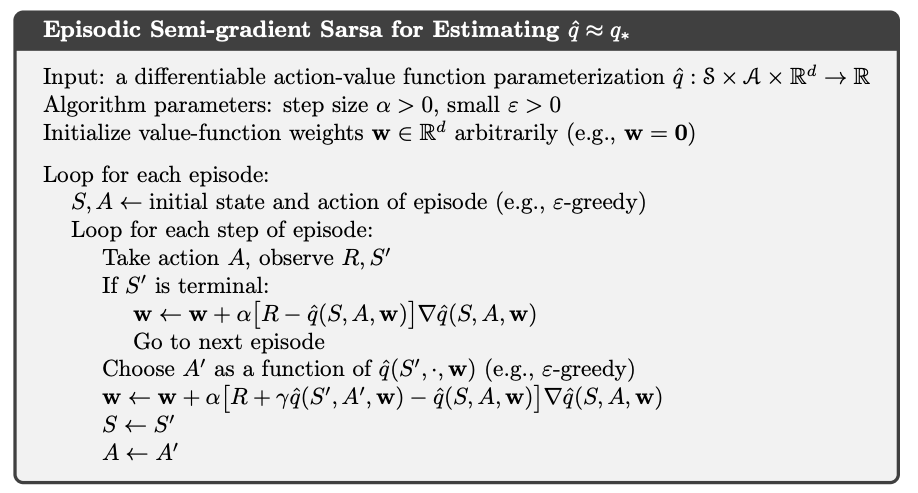
\includegraphics[width=\textwidth]{/chapter10_1}
	\caption{Episodic semi-gradient sarsa for estimating $\hat{q} \approx q_*$}
	\label{fig: 10_1}
\end{figure}

\subsection{Semi-gradient $n$-step Sarsa}
The $n$-step semi-gradient sarsa algorithm follows logically from the previous section. The $n$-step return becomes
\begin{equation}
G_{t:t+n} \doteq R_{t+1} + \gamma R_{t+2} + \cdots + \gamma^{n-1} + R_{t+n} + \gamma \hat{q}(S_{t+n}, A_{t+n}, \textbf{w}_{t+n-1})
\end{equation}

The $n$-step update becomes
\begin{equation}
\textbf{w}_{t+n} \doteq \textbf{w}_{t+n-1} + \alpha \left[G_{t:t+n} - \hat{q} (S_t, A_t, \textbf{w}_{t+n-1})\right] \nabla \hat{q}(S_t, A_t, \textbf{w}_{t+n-1})
\end{equation}

The algorithm is provided in Figure \ref{fig: 10_2}. Generally, an intermediate level of bootstrapping shows optimal performance.

\begin{figure}[h!]
	\centering
	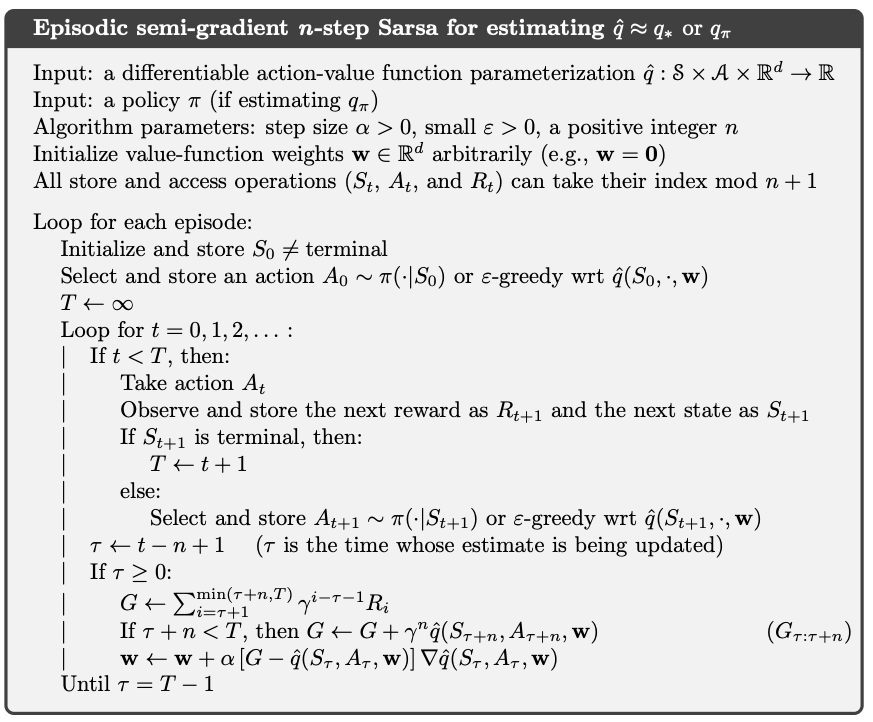
\includegraphics[width=0.8\textwidth]{/chapter10_2}
	\caption{Episodic semi-gradient $n$-step sarsa for estimating $\hat{q} \approx q_*$}
	\label{fig: 10_2}
\end{figure}

\subsection{Average Reward: A New Problem Setting for Continuing Tasks}
Until now we have considered two types of rewards: episodic and discounted (for continuing tasks). The average reward is a third task with no discounting, such that future rewards are valued just the same as present rewards. In the average-reward setting, the quality of a policy $\pi$ is defined as the average rate of reward, or simply \textit{average reward}, while following that policy, which we denote as $r(\pi)$
\begin{align}
r(\pi) &\doteq \lim_{h \rightarrow \infty}\frac{1}{h} \sum_{t=1}^{h} \mathbb{E} \left[R_t | S_0, A_{0:t-1} ~ \pi \right] \\
&= \lim_{t \rightarrow \infty} \mathbb{E} \left[R_t | S_0, A_{0:t-1} ~ \pi \right] \\
&= \sum_{s} \mu_\pi(s) \sum_{a} \pi(a|s) \sum_{s', r} p(s', r|s,a)r
\end{align}

The last equation holds if $\mu_\pi(s)$ exists and is independent of $S_0$, in other words if the MDP is \textit{ergodic} i.e. the long run expectation of being in a state depends only on the policy and the MDP transition probabilities.

We can order policies based on their average reward per timestep–$r(\pi)$– and all policies that attain the maximal reward rate are considered optimal.

In the average-reward setting, returns are defined in terms of differences between rewards and the average reward
\begin{equation}
G_t \doteq R_{t+1} - r(\pi) + R{t+2} - r(\pi) + R{t+3} - r(\pi) + \cdots
\end{equation}
known as the \textit{differential return} with corresponding value functions known as \textit{differential value functions}. This can be used to create new TD errors, the action-value error being
\begin{equation}
\delta_t \doteq R_{t+1} - \bar{R}_t + \hat{q}(S_{t+1}, A_{t+1}, \textbf{w}_t) - \hat{q}(S_t, A_t, \textbf{w}_t)
\end{equation}

where $\bar{R}_t$ is an estimate at time $t$ of the average reward $r(\pi)$. This error can be used to create a differential semi-gradient sarsa algorithm as shown in Figure \ref{fig: 10_3}
\begin{figure}[h!]
	\centering
	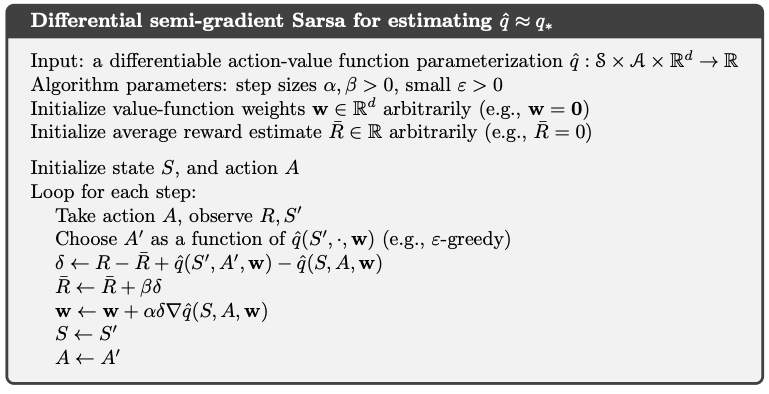
\includegraphics[width=\textwidth]{/chapter10_3}
	\caption{Differential semi-gradient sarsa for estimating $\hat{q} \approx q_*$}
	\label{fig: 10_3}
\end{figure}

\subsection{Deprecating the Discounted Setting}
Should we use the discounted reward or the average reward in continuous settings? It turns out there is no benefit to using discounting in the continuous setting, as, given a large enough sequences of rewards (infinite in the limit) we end up multiplying every reward by the same sequence of discounts $1 + \gamma + \gamma^2 + \gamma^3 + \gamma^4 + \cdots = \frac{1}{1 - \gamma}$.

The root cause of difficulties with the discounted control setting is that with function approximation we lose the policy improvement theorem from chapter 4. We can no longer say that if we change the policy to improve the discounted value of one state we are guaranteed to have improved the overall policy - errors in our function approximation mean we could have a detrimental effect on our value function elsewhere.

\subsection{Differential Semi-gradient $n$-step Sarsa}
For the $n$-step generalisation of Sarsa, we just need an expression for the $n$-step differential return with function approximation:
\begin{equation}
G_{t:t+n} \doteq R_{t+1} - \bar{R}_{t+n-1} + \cdots + R_{t+n} - \bar{R}_{t+n-1} - \hat{q}(S_{t+n}, A_{t+n}, \textbf{w}_{t+n-1}) 
\end{equation}

The pseudocode is given in Figure \ref{fig: 10_4}.

\begin{figure}[h!]
	\centering
	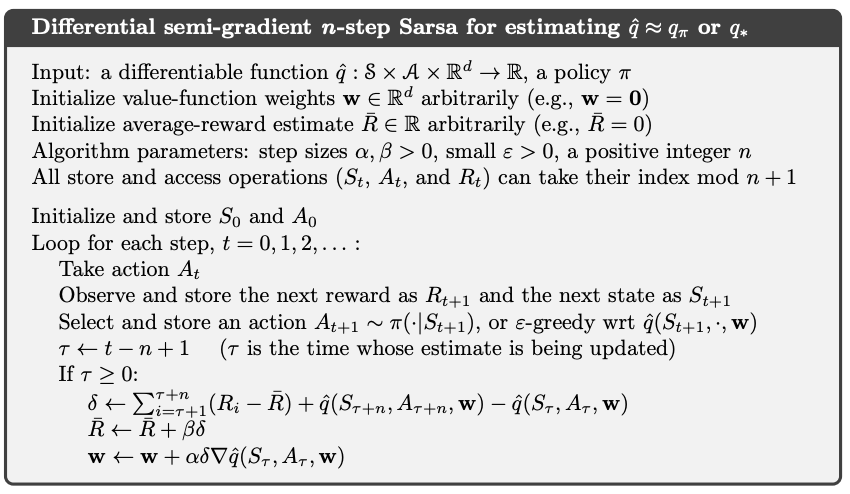
\includegraphics[width=\textwidth]{/chapter10_4}
	\caption{Differential semi-gradient $n$-step sarsa for estimating $\hat{q} \approx q_*$}
	\label{fig: 10_4}
\end{figure}

\subsection{Key Takeaways}
\begin{itemize}
\item In the episodic case, control with function approximation works the same as before, we find the approximate value function and act greedily.
\item In the continuing task setting we need to introduce a new reward–the average reward $r(\pi)$–which represents our expectation over the reward space.
\item Our updates are now governed by the \textit{differential reward} which is the difference between our observed reward and current best estimate for the average reward.
\item Discounting does not matter/work in the presence of approximations, as in this case, most policies cannot be represented by a value function. Instead, policies need to be ranked and the average reward $r(\pi)$ provides an effective way to do this.
\end{itemize}





\section{*Off-policy Methods with Approximation}
Notes on this section tbc.
\documentclass[a4paper, oneside, 11pt]{article}
\usepackage[margin=2.5cm]{geometry}
\usepackage{amssymb}
\usepackage{amsmath}
\usepackage{graphicx}
\usepackage{bm}
\usepackage{mathtools}
\usepackage{setspace}
\usepackage{dsfont}
\usepackage{xcolor}
\usepackage{upquote}
\usepackage[utf8]{inputenc}
\usepackage[colorlinks=true, linkcolor=black, urlcolor=blue, citecolor=black]{hyperref}

\usepackage[shortlabels]{enumitem}

\setlength{\parindent}{0cm}

\newcommand\Rule{\noindent\makebox[\textwidth]{\rule{\textwidth}{0.5pt}}}

\newcommand\argmax{\operatorname*{argmax}}
\newcommand\argmin{\operatorname*{argmin}}

\renewcommand{\vec}[1]{\boldsymbol{#1}}

\newcommand{\R}{\mathbb{R}}
\newcommand\Epi{\mathbb{E}_{\pi}}
\renewcommand\P{\mathbb{P}}
\newcommand\E{\mathbb{E}}
\newcommand{\VE}{\overline{\mathrm{VE}}}

\renewcommand{\S}{\mathcal{S}}
\newcommand{\A}{\mathcal{A}}
\newcommand{\grad}{\nabla}
\renewcommand{\d}{\mathrm{d}}


\renewcommand{\familydefault}{\sfdefault}


\newcommand\RepoAddress{https://github.com/brynhayder/reinforcement_learning_an_introduction}
\newcommand\RepoName{github.com/brynhayder/reinforcement\_learning\_an\_introduction}

\newcommand\ProjectDir{/Users/Bryn/Programming/remote/ReinforcementLearningAnIntroduction}
\newcommand\NotesImages{\ProjectDir/data/notes_images}
\newcommand\ExerciseOutput{\ProjectDir/data/exercise_output}

\newcommand\ProgrammingExercise{This is a programming exercise. For the relevant code please see \href{\RepoAddress{}}{the repo}.}



\begin{document}
    \section{Eligibility Traces}
\end{document}
\section{Policy Gradient Methods}
Instead of learning action-value estimates, and deriving a policy thereafter, we will now parameterize a policy directly depending on its performance. Our policy is now $\pi(a|s, \boldsymbol{\theta})$ representing the probability of taking action $a$ in state $s$ given parameter vector $\theta \in \mathbb{R}^{d'}$. \textit{Actor-critic} methods learn both a parameterised policy (the actor) and a parameterised value function estimate (the critic)

The policy parameter update is therefore
\begin{equation}
\boldsymbol{\theta}_{t+1} = \boldsymbol{\theta}_{t} + \alpha \nabla \hat{J(\boldsymbol{\theta}_{t})} 
\end{equation}

where $\hat{J(\boldsymbol{\theta}_{t})}$ is a stochastic estimate whose expectation approximates the gradient of the performance measure with respect to its argument $\boldsymbol{\theta}_{t}$.

\subsection{Policy Approximation and its Advantages}
\begin{itemize}

\item The policy can be parameterised in any way as long as $\pi(a|s, \boldsymbol{\theta})$ is differentiable.
\item If the action-space is discrete and not too large, then a natural and common kind of parameterisation is to form numerical preferences $h(s,a, \boldsymbol{\theta}) \in \mathbb{R}$ for each state-action pair. The actions with the highest preferences in each state are given the highest probabilities of being selected, for example, according to an exponential soft-max distribution:
\begin{equation}
\pi(a|s, \boldsymbol{\theta}) \doteq \frac{e^{h(s,a,\boldsymbol{\theta})}}{\sum_{b}e^{h(s,b,\boldsymbol{\theta})}}
\end{equation}.

\item We call this kind of policy parameterisation \textit{soft-max in action preferences}. An advantage of parameterising policies according to soft-max action preferences is that the approximate policy can approach a determinisitc policy, whereas with $\epsilon$-greedy action selection over action values there is always an $\epsilon$ probability of selecting a random action.
\item A second advantage of soft-max action preferences is that we can now select actions with arbritrary probabilities, rather than the greedy action selected most of the time and all other actions given probability of selection $\epsilon / |\mathcal{A}|$. This is useful in environments with imperfect information, where it is useful to act stochastically e.g. when bluffing in poker it is useful to do so randomly to unnerve an opponent.
\item Often the most important reason for using a policy-gradient method is that we can inject prior knowledge about the system in the RL agent.
\end{itemize}

\subsection{The Policy Gradient Theorem}
We define performance in the episodic case as
\begin{equation}
J(\boldsymbol{\theta}) \doteq v_{\pi\theta(s_0)},
\end{equation}
where $v_{\pi\theta(s_0)}$ is the true value function for $\pi_{\boldsymbol{\theta}}$, the policy determined by $\boldsymbol{\theta}$. And $s_0$ is some non-random start state. The policy gradient theorem then establishes that
\begin{equation} \label{eq: policy gradient theorem}
\nabla J(\boldsymbol{\theta}) \propto \sum_{s} \mu(s) \sum_{a} q_\pi(s,a) \nabla \pi(a|s, \boldsymbol{\theta})
\end{equation}

where $\mu$ is the on-policy distribution under $\pi$ as discussed previously i.e. the theorem is a sum over states weighted by how often the states occur under the target policy $\pi$. We can use this to approximate gradient ascent without access to the derivative of the state distribution.

\subsection{REINFORCE: Monte Carlo Policy Gradient}
REINFORCE is a method for updating our policy parameters based on episodic returns from states $G_t$. We update the parameters in the direction of actions that yielded highest rewards. Recall from Equation \ref{eq: policy gradient theorem} that the policy gradient theorem is a weighted sum of over states which is the same as an expectation over states:
\begin{align}
\nabla J(\boldsymbol{\theta}) &\propto \sum_{s} \mu(s) \sum_{a} q_\pi(s,a) \nabla \pi(a|s, \boldsymbol{\theta}) \\
&= \mathbb{E}_\pi \left[\sum_{a} q_\pi(S_t, a) \nabla \pi(a, S_t, \boldsymbol{\theta})  \right]
\end{align}

We can arrive at REINFORCE by replacing the sum over the random variable's possible values by an expectation under $\pi$, and then sampling the expectation. We multiply and divide the summed terms by $\pi(a | S_t, \boldsymbol{\theta})$:
\begin{align}
\nabla J(\boldsymbol{\theta}) &\propto \mathbb{E}_\pi \left[\sum_{a} \pi(a | S_t, \boldsymbol{\theta}) q_\pi(S_t, a) \frac{\nabla \pi(a, S_t, \boldsymbol{\theta})}{\pi(a, S_t, \boldsymbol{\theta})} \right] \\
&= \mathbb{E}_\pi \left[q_\pi(S_t, A_t) \frac{\nabla \pi(A_t, S_t, \boldsymbol{\theta})}{\pi(A_t, S_t, \boldsymbol{\theta})} \right] \; \; \; \text{(replacing $a$ by the sample $A_t \sim \pi$)} \\
&= \mathbb{E}_\pi \left[G_t \frac{\nabla \pi(A_t, S_t, \boldsymbol{\theta})}{\pi(A_t, S_t, \boldsymbol{\theta})} \right] \; \; \; \text{(because $\mathbb{E}_\pi \left[G_t|S_t, A_t\right] = q_\pi(S_t, A_t)$)} \\
\end{align}

The last expression is what we need: a quantity that can be sampled on each time step whose expectation is proportional to the gradient. We now arrive at the REINFORCE update
\begin{equation}
\boldsymbol{\theta}_{t+1} \doteq \boldsymbol{\theta}_{t} + \alpha G_t \frac{\nabla \pi(A_t, S_t, \boldsymbol{\theta})}{\pi(A_t, S_t, \boldsymbol{\theta})}
\end{equation}

This update makes intuitive sense. The gradient term represents the direction in parameter space that most increases the probability of taking that same action again in the future. In effect, the gradient distil the policy approximation down to the weights that were most responsible for the action taken, from there we can affect these weights based on how much we valued the action. If the action yielded high reward $G_t$, then we boost the weights in proportion to the reward, and if this action has low probability of being taken under the current policy (the denominator $\pi(A_t, S_t, \boldsymbol{\theta})$) then the weights are further boosted. Alternatively, if the action is taken often, and yields low reward, we make little adjustment to the weights, lowering their impact on the policy approximation in the long run as other weights receive boosts.

Note this is a monte carlo algorithm, using complete returns as updates, meaning it is only well defined in the episodic case, and can have high variance causing slow learning. The pseudocode for REINFORCE is given in Figure \ref{fig: 13_1}.
\begin{figure}
	\centering
	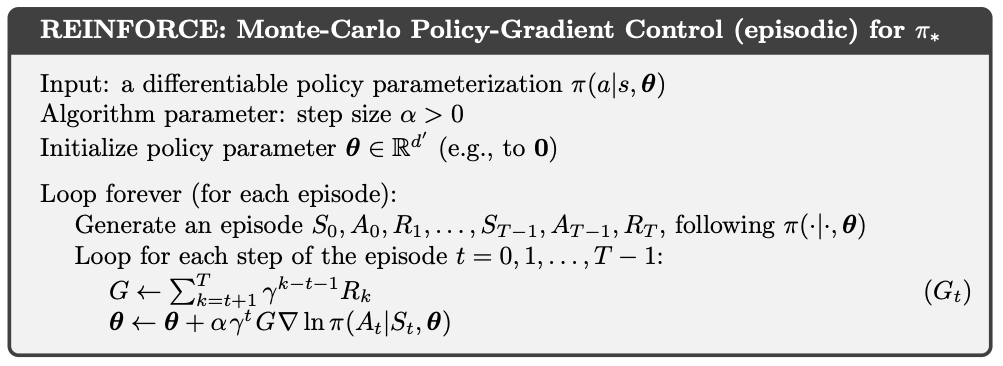
\includegraphics[width=\textwidth]{/chapter13_1}
	\caption{Pseudocode for REINFORCE: monte carlo policy-gradient control (episodic) for $\pi_*$}
	\label{fig: 13_1}
\end{figure}

\subsection{REINFORCE with Baseline}
The policy gradient theorem can be generalized to include a comparison of the action value to an arbitrary \textit{baseline} $b(s)$:
\begin{equation}
\nabla J(\boldsymbol{\theta}) \propto \sum_{s} \mu(s) \sum_{a} \left( q_\pi(s,a) - b(s) \right) \nabla \pi(a|s, \boldsymbol{\theta})
\end{equation}

We do this because it can help us reduce the variance of our results, which speeds learning. By comparing our observed result with some state-dependent baseline, we get a feel for how different the observed value is from what we expected. Thus, we arrive at a lower variance REINFORCE update as
\begin{equation}
\boldsymbol{\theta}_{t+1} \doteq \boldsymbol{\theta}_{t} + \alpha \left(G_t - b(S_t) \right) \frac{\nabla \pi(A_t, S_t, \boldsymbol{\theta})}{\pi(A_t, S_t, \boldsymbol{\theta})}
\end{equation}

The natural baseline is an estimate of the state value, $\hat{v}(S_t, \textbf{w})$, which we can learn as discussed in previous chapters. This method significantly speeds up learning as shown in Figure \ref{fig: 13_2}.
\begin{figure}
	\centering
	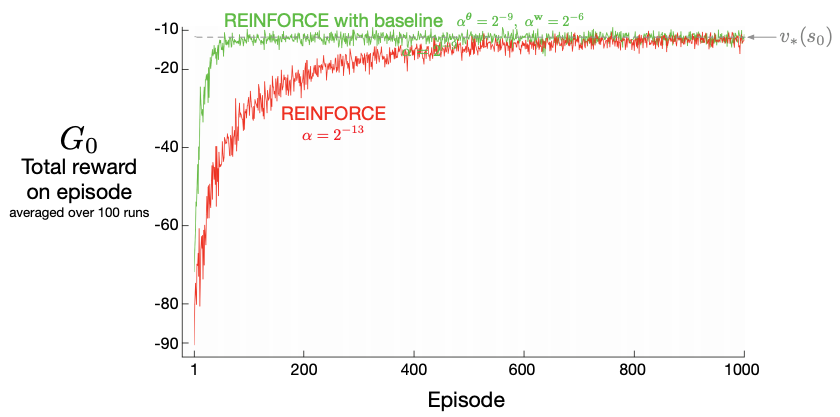
\includegraphics[width=\textwidth]{/chapter13_2}
	\caption{Adding a baseline to REINFORCE can make it learn much faster, as illustrated here on the short-corridor gridworld (Example 13.1). The step size used here for plain REINFORCE is that at which it performs best.}
	\label{fig: 13_2}
\end{figure}

\subsection{Actor-Critic Methods}
\begin{itemize}
\item The REINFORCE method uses the state-value function as a baseline for comparing true return from a state with what we expected the return to be. Because this comparison is made prior to action selection, we cannot use it to directly evaluate actions. In actor-critic methods, the state-value function is applied also to the \textit{second} state of the transition, which, when discounted and added to the one-step reward, constitutes the one-step return $G_{t:t+1}$.
\item When the state-value function is used in this way it is called the \textit{critic} and the policy is the \textit{actor}.
\item One-step actor-critic methods replace the full return of REINFORCE with the one-step return (and use a learned state-value function as the baseline) as follows:
\begin{align}
\boldsymbol{\theta}_{t+1} &\doteq \boldsymbol{\theta}_{t} + \alpha \left(G_{t:t+1} - \hat{v}(S_t, \textbf{w}) \right) \frac{\nabla \pi(A_t, S_t, \boldsymbol{\theta})}{\pi(A_t, S_t, \boldsymbol{\theta})} \\
&=  \boldsymbol{\theta}_{t} + \alpha \left(R_{t+1} + \gamma \hat{v}(S_{t+1}, \textbf{w}) - \hat{v}(S_t, \textbf{w})  \right) \frac{\nabla \pi(A_t, S_t, \boldsymbol{\theta})}{\pi(A_t, S_t, \boldsymbol{\theta})} \\
&=  \boldsymbol{\theta}_{t} + \alpha \delta_t \frac{\nabla \pi(A_t, S_t, \boldsymbol{\theta})}{\pi(A_t, S_t, \boldsymbol{\theta})} 
\end{align}
\item The pseudocode for one-step actor-critic is given in Figure \ref{fig: 13_3}, and it can be extended to include eligibility traces from Chapter 11 as shown in Figure \ref{fig: 13_4}.
\end{itemize}

\begin{figure}
	\centering
	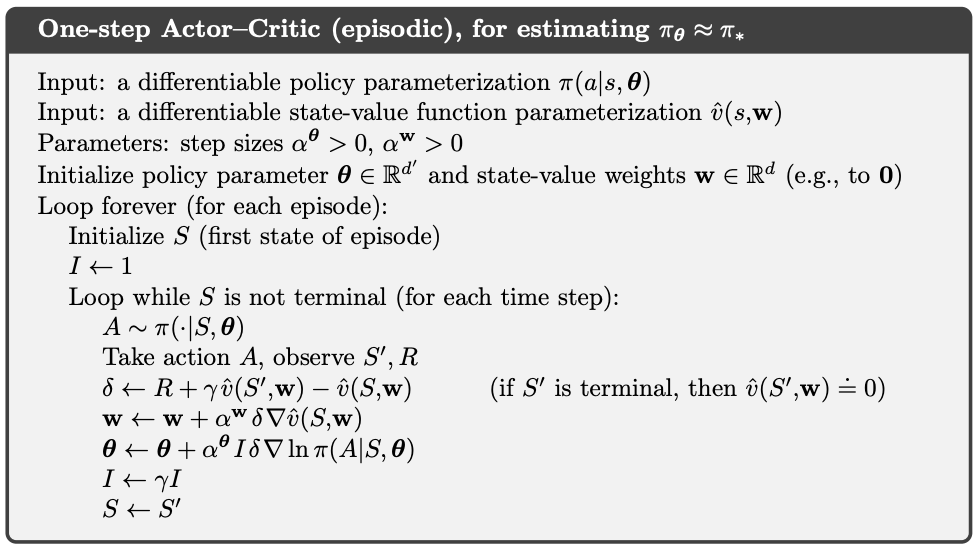
\includegraphics[width=0.8\textwidth]{/chapter13_3}
	\caption{Pseudocode for one-step actor-critic}
	\label{fig: 13_3}
\end{figure}

\begin{figure}
	\centering
	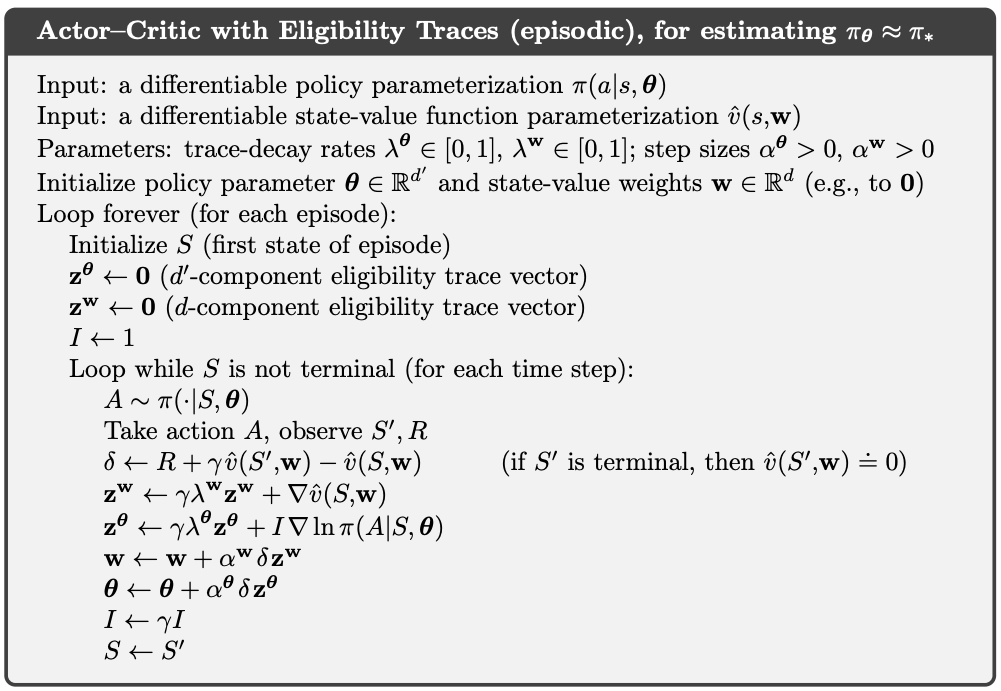
\includegraphics[width=0.8\textwidth]{/chapter13_4}
	\caption{Pseudocode for one-step actor-critic with eligibility traces}
	\label{fig: 13_4}
\end{figure}

\subsection{Policy Gradient for Continuing Problems}
As discussed in Chapter 10, for continuing problems without episode boundaries we need to define the performance in terms of average rate of reward per time step:
\begin{align}
J(\boldsymbol{\theta}) &\doteq r(\pi) \\
&= \lim_{t \rightarrow \infty} \mathbb{E} [R_t | S_0, A_{0:t-1} \sim \pi] \\
&= \sum_{s} \mu(s) \sum_{a} \pi(a | s) \sum_{s', r} p(s', r | s, a) r \\ 
\end{align}

We need to remember that in the continuing case, we define values $v_\pi(s) \doteq \mathbb{E}[G_t, S_t = s]$ and $q_\pi(s,a) \doteq \mathbb{E}[G_t, S_t = s, A_t = a]$ w.r.t the differential return:
\begin{equation}
G_t \doteq R_{t+1} - r(\pi) + R_{t+2} - r(\pi) + R_{t+3} - r(\pi) + \cdots
\end{equation}
Pseudocode for the continuing case is given in Figure \ref{fig: 13_5}.

\begin{figure}
	\centering
	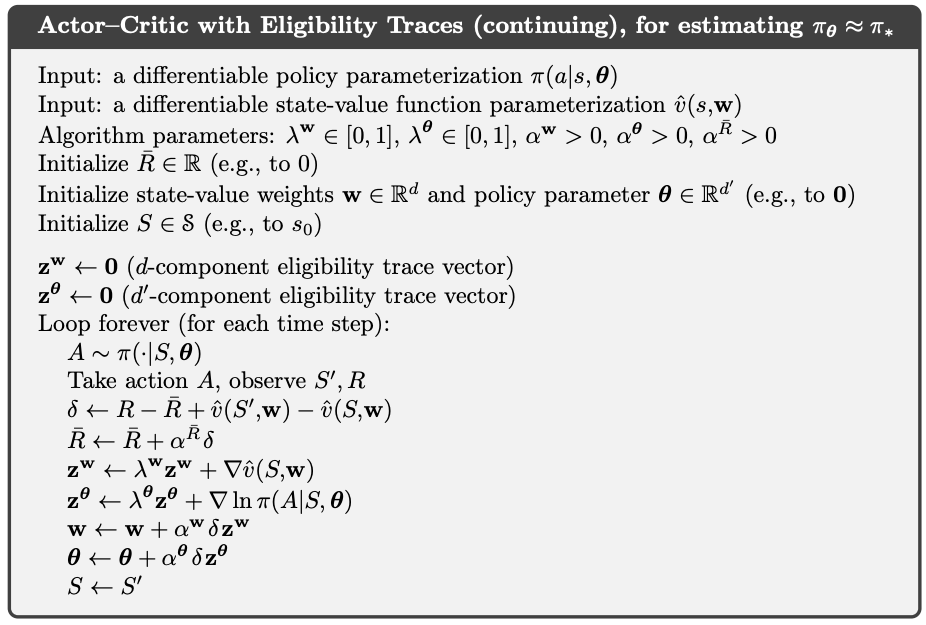
\includegraphics[width=0.8\textwidth]{/chapter13_5}
	\caption{Pseudocode for one-step actor-critic with eligibility traces, continuing case}
	\label{fig: 13_5}
\end{figure}

\subsection{Policy Parameterisation for Continuous Actions}
For state-spaces with huge numbers of actions, or continuous action spaces with infinite numbers of actions, we do not need to learn the probability of selecting each of these many actions, we can instead learn the parameters of the distribution over actions given a state. The probability density function for the normal distribution is conventionally written
\begin{equation}
p(x) \doteq \frac{1}{\sigma \sqrt{2 \pi}}exp\left(-\frac{(x - \mu)^2}{2 \sigma^2}\right)
\end{equation}

where $\mu$ and $\sigma$ are the mean and standard deviation of the normal distribution. Note $p(x)$ is the density of the probability, \textit{not} the probability itself. As such it can be greater than 1; it is the area under the graph that must sum to 1. One can take the integral between two values of $x$ to arrive at the probability of $x$ falling within that range. The policy parameterisation therefore becomes:
\begin{equation}
\pi(a | s, \boldsymbol{\theta}) \doteq \frac{1}{\sigma(s, \boldsymbol{\theta}) \sqrt{2 \pi}}exp\left(-\frac{(x - \mu(s, \boldsymbol{\theta}))^2}{2 \sigma(s, \boldsymbol{\theta})^2}\right)
\end{equation}

where $\mu : \mathcal{S} \times \mathbb{R}^{d'} \rightarrow \mathbb{R}$ and $\sigma : \mathcal{S} \times \mathbb{R}^{d'} \rightarrow \mathbb{R^+}$ i.e. they are both matrices of with dimensions equal to the number of states times the number of dimensions of the feature vector defining the policy. To from the policy approximator we need to split the policy's parameter vector into two parts, $\boldsymbol{\theta} = [\boldsymbol{\theta}_\mu, \boldsymbol{\theta}_\sigma]^T$. The mean can be approximated as a linear function, but the standard deviation must always be positive and is better approximated as the exponential of a linear function. Thus
\begin{equation}
\mu(s, \boldsymbol{\theta}) \doteq \boldsymbol{\theta}_\mu^T \textbf{x}_\mu(s) \; \; \; \text{and} \; \; \; \sigma(s, \boldsymbol{\theta}) \doteq exp\left(\boldsymbol{\theta}_\sigma^T \textbf{x}_\sigma(s)\right)
\end{equation}

\subsection{Key Takeaways}
\begin{itemize}
\item Prior to this chapter, actions had been selected by consulting an action-value function that informed us of how valuable actions were in given states at reaching our goal. Here, we instead parameterised policies directly, updating our approximations by reviewing the rewards received after taking some actions.
\item There are several advantages to doing this:
\begin{enumerate}
\item They can learn specific probabilities of taking actions (rather than sharing $\epsilon / |\mathcal{A}|)$ probability with non-greedy actions as per $\epsilon$-greedy methods)
\item They can learn appropriate levels of exploration and then approach deterministic policies in the long run
\item They can naturally handle continuous action spaces by learning distributions over actions given a state
\end{enumerate}
\item The policy gradient theorem provides a theoretical foundation for all policy gradient methods and gives an exact formula for how performance is affected by the policy parameter that does not involve derivatives of the state distribution.
\item The REINFORCE method is the policy gradient theorem in action using monte carlo returns
\item A baseline (usually our current estimate for the state-value) can be used in conjunction with REINFORCE to reduce the variance of the output and speed learning.
\item Actor-critic methods assess the policy's action selection by comparing its one-step reward with the value function at the next timestep. This introduces bias into the actor's gradient estimates, but is often desirable for the same reason that bootstrapping TD methods are often superior to Monte Carlo methods (substantially reduced variance).

\end{itemize}





\end{document}